% !TeX root = ../libro.tex
% !TeX encoding = utf8
%
%*******************************************************
% Summary
%*******************************************************

\selectlanguage{english}
\chapter{Summary}

%An english summary of the project (around 800 and 1500 words are recommended).

%File: \texttt{preliminares/summary.tex}

We begin this Bachelor's Thesis with \hyperref[ch:motivacion]{chapter 1}, which highlights the motivation behind this work, as well as the main goals to be achieved. Immediately after, in \hyperref[ch:historia]{chapter 2}, we give a brief historical contextualization of the topics covered in this writing.

The theoretical development starts in \hyperref[ch:programas-python-maquinas-turing]{chapter 3}, whose \hyperref[sec:programas-python]{section 3.1} introduces a specific subset of Python programs, namely \emph{SISO programs}, and we observe this class is as expressive as the class of all Python programs. Next, in \hyperref[sec:maquinas-turing]{section 3.2}, we delve into \emph{Turing machines}, the main mathematical tool of our analysis. In \hyperref[sec:equivalencia]{section 3.3} we introduce new and equivalent computing models, until we arrive at the main result of this chapter: the fact that Turing machines can emulate Python programs, and vice versa; in other words, Python programs and Turing machines are equivalent. This will allow us to use Python programs conveniently, instead of having to specify precise descriptions of Turing machines. We conclude the chapter introducing the Church-Turing thesis in \hyperref[sec:church-turing]{section 3.4}, and realizing that the equivalence result proved can be an argument in its favor.

We define mathematically in \hyperref[sec:problemas-decidibles]{section 4.1} the notion of \emph{computational problem}, and we discuss Python programs (and, equivalently, Turing machines), can solve them. We call \emph{decidable} any problem that can be solved by a program that never halts. In \hyperref[sec:universalidad]{section 4.2} we observe a Python program can emulate itself, which leads us in \hyperref[sec:problemas-no-decidibles]{section 4.3} to the existence of undecidable problems. In \hyperref[sec:problemas-semidecidibles]{section 4.4} we relax the halting condition to obtain \emph{semidecidable} problems. Afterwards, we introduce in \hyperref[sec:reducciones]{section 4.5} the \emph{reduction} technique, which allows us to obtain new, undecidable problems, including the most important one for this thesis in \hyperref[sec:problema-parada]{section 4.6}: the \emph{halting problem}.

In order to prove the main result of this work, it is necessary to introduce a formalization of the concepts of \emph{proof} and \emph{truth}. This is precisely what we do when introducing \emph{formal systems} \hyperref[sec:sistemas-formales]{section 4.1} and \emph{logical systems} in \hyperref[sec:sistemas-logicos]{section 4.2}. Formal systems are \emph{syntactic}: they formalize what a \emph{theorem} is, a provable \emph{formula} from a set of \emph{axioms} and \emph{inference rules}. On the other hand, logical systems incorporate to formal systems a semantic component: \emph{truth}. In \hyperref[sec:solidez-completitud-decidibilidad]{sections 5.3} and \hyperref[sec:consistencia]{5.5} we present essential properties of the aforementioned systems, which relate semantic and syntactic concepts. We highlight in \hyperref[sec:aritmetica-peano]{section 5.4} the introduction of \emph{Peano arithmetic}: a logical system of especial significance.

As colophon, we proceed to prove the First Incompleteness Theorem in \hyperref[ch:teorema-incompletitud]{chapter 6}: we do so first from Peano arithmetic in \hyperref[sec:primera-aproximacion]{section 6.1}, and then we generalize it by means of two versions. The first one, of a semantic nature, is proven in \hyperref[sec:version-semantica]{section 6.2}, and allows us (under some computational hypotheses) to find true but unprovable statements in a logical system. Next, the syntactic version of \hyperref[sec:version-sintactica]{section 6.3}, closer to Gödel's, allows us to find unprovable statements in formal systems. We finish the study of this theorem in \hyperref[sec:consecuencias]{section 6.4}, with some important mathematical (\hyperref[subsec:segundo-problema-hilbert]{section 6.4.1}) and philosophical (\hyperref[subsec:mente-humana-tesis-church-turing]{section 6.4.2}) consequences.

Finally, we wrap up with some conclusions in \hyperref[ch:conclusiones]{chapter 7}, and some final words for further work in \hyperref[ch:trabajo-futuro]{chapter 8}.

%\vfill
% ====================
\begin{sidewaysfigure}
\centering
%\vspace{8pt}
%\hspace*{-1cm}


\tikzset{every picture/.style={line width=0.75pt}} %set default line width to 0.75pt        

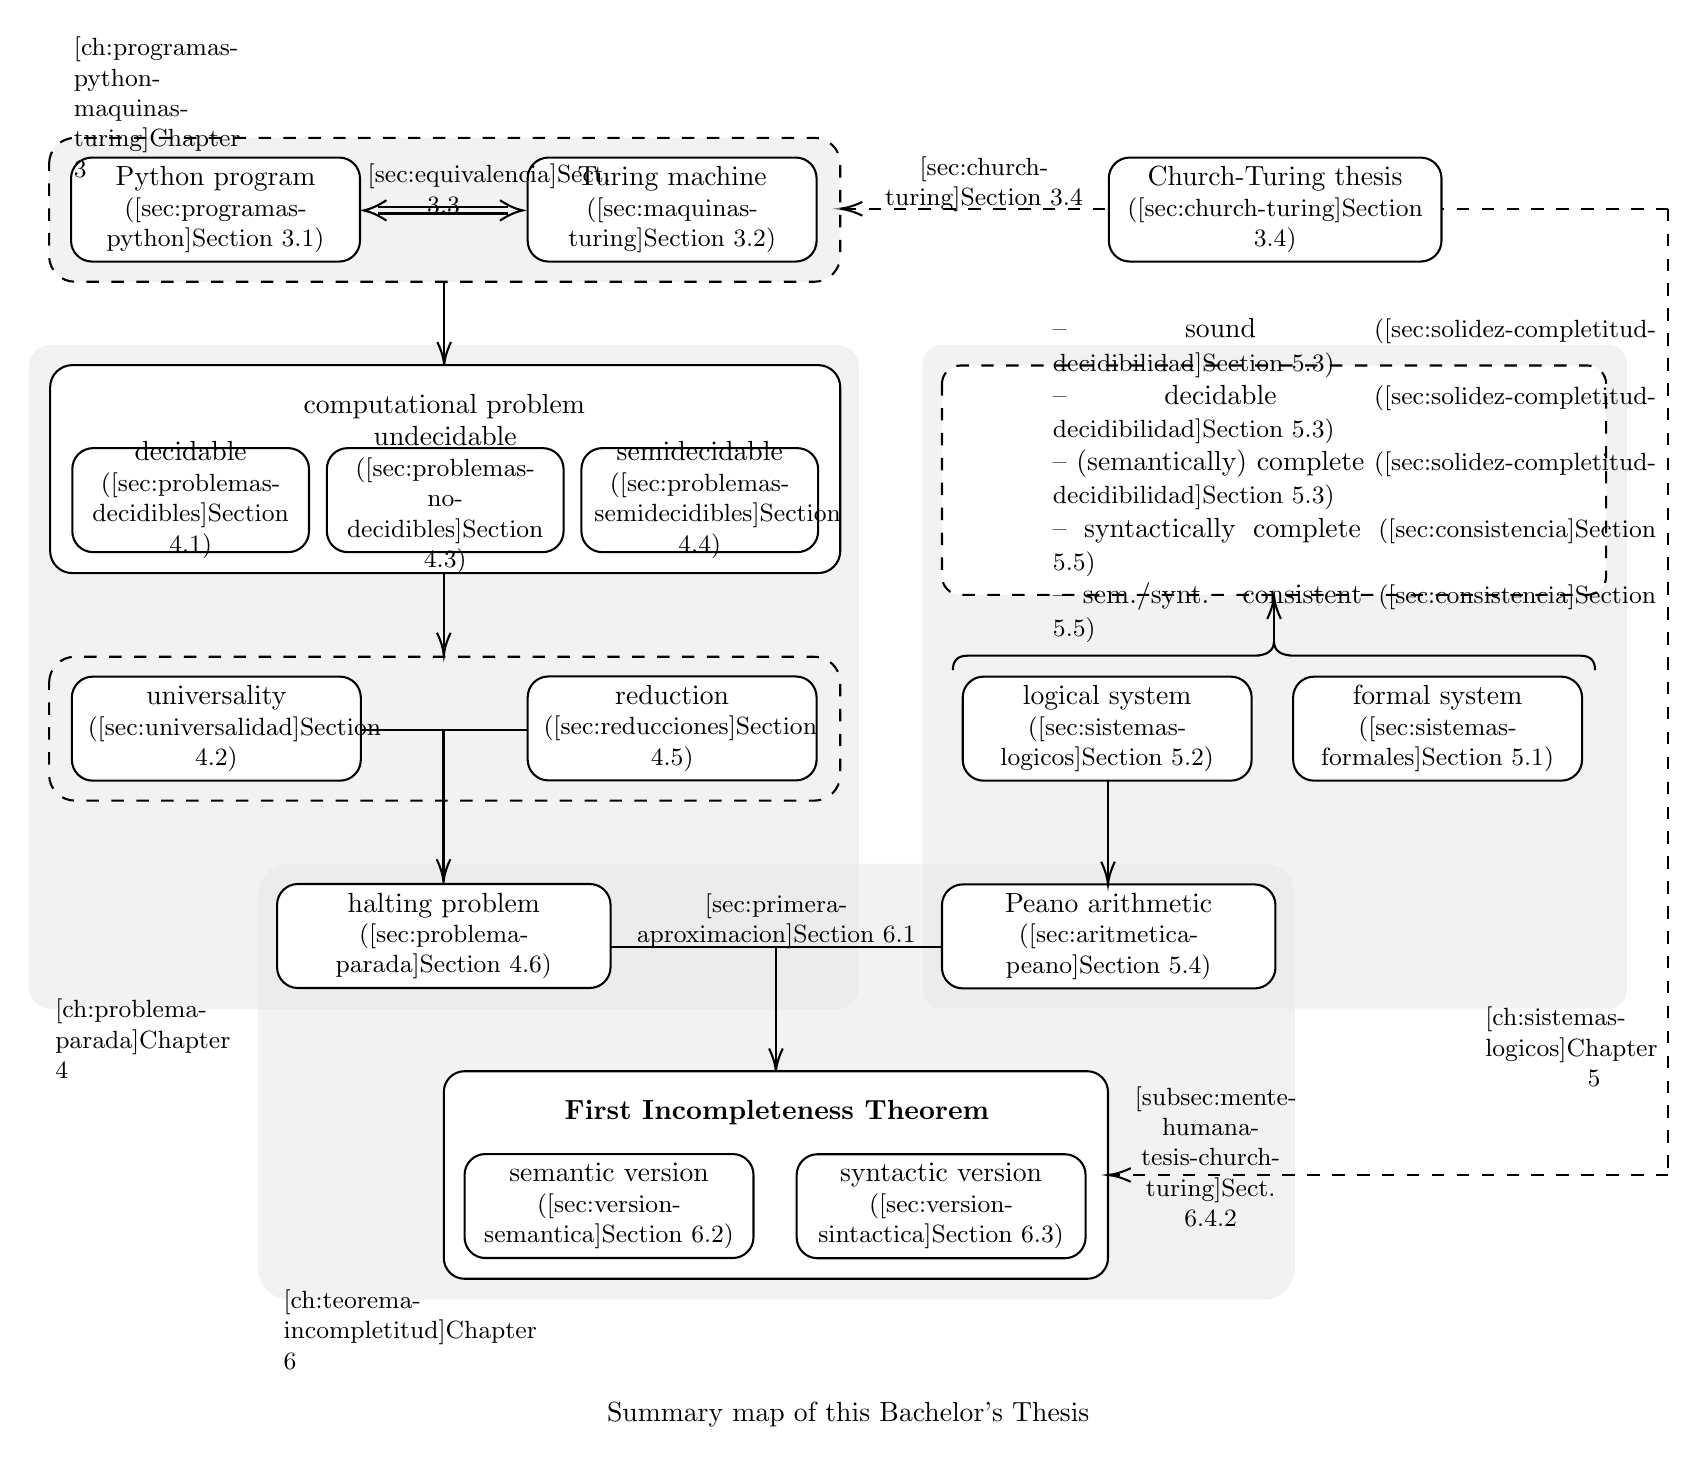
\begin{tikzpicture}[x=0.75pt,y=0.75pt,yscale=-1,xscale=1]
%uncomment if require: \path (0,694); %set diagram left start at 0, and has height of 694

%Straight Lines [id:da2056540562354816] 
\draw  [dash pattern={on 4.5pt off 4.5pt}]  (672,64.47) -- (810,64.47) ;
%Straight Lines [id:da23044041717189923] 
\draw  [dash pattern={on 4.5pt off 4.5pt}]  (412.67,64.47) -- (610,64.47) ;
\draw [shift={(410.67,64.47)}, rotate = 0] [color={rgb, 255:red, 0; green, 0; blue, 0 }  ][line width=0.75]    (10.93,-3.29) .. controls (6.95,-1.4) and (3.31,-0.3) .. (0,0) .. controls (3.31,0.3) and (6.95,1.4) .. (10.93,3.29)   ;
%Straight Lines [id:da8398435684999113] 
\draw  [dash pattern={on 4.5pt off 4.5pt}]  (810,64.47) -- (810,530) ;
%Rounded Rect [id:dp027018508739026448] 
\draw  [draw opacity=0][fill={rgb, 255:red, 230; green, 230; blue, 230 }  ,fill opacity=0.5 ] (20,439.33) .. controls (20,445.22) and (24.78,450) .. (30.67,450) -- (409.33,450) .. controls (415.22,450) and (420,445.22) .. (420,439.33) -- (420,140.67) .. controls (420,134.78) and (415.22,130) .. (409.33,130) -- (30.67,130) .. controls (24.78,130) and (20,134.78) .. (20,140.67) -- cycle ;
%Rounded Rect [id:dp9415679498487528] 
\draw  [dash pattern={on 4.5pt off 4.5pt}] (29.83,292.77) .. controls (29.83,285.88) and (35.41,280.3) .. (42.3,280.3) -- (398.54,280.3) .. controls (405.42,280.3) and (411,285.88) .. (411,292.77) -- (411,337.17) .. controls (411,344.05) and (405.42,349.64) .. (398.54,349.64) -- (42.3,349.64) .. controls (35.41,349.64) and (29.83,344.05) .. (29.83,337.17) -- cycle ;
%Rounded Rect [id:dp05100022295548956] 
\draw  [draw opacity=0][fill={rgb, 255:red, 230; green, 230; blue, 230 }  ,fill opacity=0.5 ] (130.5,575) .. controls (130.5,583.28) and (137.22,590) .. (145.5,590) -- (615,590) .. controls (623.28,590) and (630,583.28) .. (630,575) -- (630,395) .. controls (630,386.72) and (623.28,380) .. (615,380) -- (145.5,380) .. controls (137.22,380) and (130.5,386.72) .. (130.5,395) -- cycle ;
%Rounded Rect [id:dp6496809750851564] 
\draw  [draw opacity=0][fill={rgb, 255:red, 230; green, 230; blue, 230 }  ,fill opacity=0.5 ] (450.61,440.79) .. controls (450.61,445.82) and (454.69,449.9) .. (459.72,449.9) -- (780.89,449.9) .. controls (785.92,449.9) and (790,445.82) .. (790,440.79) -- (790,139.11) .. controls (790,134.08) and (785.92,130) .. (780.89,130) -- (459.72,130) .. controls (454.69,130) and (450.61,134.08) .. (450.61,139.11) -- cycle ;
%Rounded Rect [id:dp549636265291094] 
\draw  [fill={rgb, 255:red, 230; green, 230; blue, 230 }  ,fill opacity=0.5 ][dash pattern={on 4.5pt off 4.5pt}] (29.83,42.77) .. controls (29.83,35.88) and (35.41,30.3) .. (42.3,30.3) -- (398.54,30.3) .. controls (405.42,30.3) and (411,35.88) .. (411,42.77) -- (411,87.17) .. controls (411,94.05) and (405.42,99.64) .. (398.54,99.64) -- (42.3,99.64) .. controls (35.41,99.64) and (29.83,94.05) .. (29.83,87.17) -- cycle ;
%Rounded Rect [id:dp1378581119146769] 
\draw  [fill={rgb, 255:red, 255; green, 255; blue, 255 }  ,fill opacity=1 ] (40.4,49.82) .. controls (40.4,44.29) and (44.89,39.8) .. (50.42,39.8) -- (169.58,39.8) .. controls (175.11,39.8) and (179.6,44.29) .. (179.6,49.82) -- (179.6,79.88) .. controls (179.6,85.41) and (175.11,89.9) .. (169.58,89.9) -- (50.42,89.9) .. controls (44.89,89.9) and (40.4,85.41) .. (40.4,79.88) -- cycle ;
%Straight Lines [id:da8729153203483555] 
\draw    (188.42,63.77) -- (250.99,63.77)(188.42,66.77) -- (250.99,66.77) ;
\draw [shift={(257.99,65.27)}, rotate = 180] [color={rgb, 255:red, 0; green, 0; blue, 0 }  ][line width=0.75]    (10.93,-4.9) .. controls (6.95,-2.3) and (3.31,-0.67) .. (0,0) .. controls (3.31,0.67) and (6.95,2.3) .. (10.93,4.9)   ;
\draw [shift={(181.42,65.27)}, rotate = 0] [color={rgb, 255:red, 0; green, 0; blue, 0 }  ][line width=0.75]    (10.93,-4.9) .. controls (6.95,-2.3) and (3.31,-0.67) .. (0,0) .. controls (3.31,0.67) and (6.95,2.3) .. (10.93,4.9)   ;
%Straight Lines [id:da845243590120559] 
\draw    (220.17,99.97) -- (220.17,137.64) ;
\draw [shift={(220.17,139.64)}, rotate = 270] [color={rgb, 255:red, 0; green, 0; blue, 0 }  ][line width=0.75]    (10.93,-3.29) .. controls (6.95,-1.4) and (3.31,-0.3) .. (0,0) .. controls (3.31,0.3) and (6.95,1.4) .. (10.93,3.29)   ;
%Straight Lines [id:da7497001546502899] 
\draw    (380,420.33) -- (380,478) ;
\draw [shift={(380,480)}, rotate = 270] [color={rgb, 255:red, 0; green, 0; blue, 0 }  ][line width=0.75]    (10.93,-3.29) .. controls (6.95,-1.4) and (3.31,-0.3) .. (0,0) .. controls (3.31,0.3) and (6.95,1.4) .. (10.93,3.29)   ;
%Straight Lines [id:da5689893955334542] 
\draw    (300,420) -- (460,420) ;
%Rounded Rect [id:dp18582062333838767] 
\draw  [fill={rgb, 255:red, 255; green, 255; blue, 255 }  ,fill opacity=1 ] (260.4,49.82) .. controls (260.4,44.29) and (264.89,39.8) .. (270.42,39.8) -- (389.58,39.8) .. controls (395.11,39.8) and (399.6,44.29) .. (399.6,49.82) -- (399.6,79.88) .. controls (399.6,85.41) and (395.11,89.9) .. (389.58,89.9) -- (270.42,89.9) .. controls (264.89,89.9) and (260.4,85.41) .. (260.4,79.88) -- cycle ;
%Rounded Rect [id:dp9523169763067778] 
\draw  [fill={rgb, 255:red, 255; green, 255; blue, 255 }  ,fill opacity=1 ] (470,299.92) .. controls (470,294.39) and (474.49,289.9) .. (480.02,289.9) -- (599.18,289.9) .. controls (604.71,289.9) and (609.2,294.39) .. (609.2,299.92) -- (609.2,329.98) .. controls (609.2,335.51) and (604.71,340) .. (599.18,340) -- (480.02,340) .. controls (474.49,340) and (470,335.51) .. (470,329.98) -- cycle ;
%Rounded Rect [id:dp48544030815291705] 
\draw  [fill={rgb, 255:red, 255; green, 255; blue, 255 }  ,fill opacity=1 ] (220,490) .. controls (220,484.48) and (224.48,480) .. (230,480) -- (530,480) .. controls (535.52,480) and (540,484.48) .. (540,490) -- (540,570) .. controls (540,575.52) and (535.52,580) .. (530,580) -- (230,580) .. controls (224.48,580) and (220,575.52) .. (220,570) -- cycle ;
%Rounded Rect [id:dp08222627508455749] 
\draw  [fill={rgb, 255:red, 255; green, 255; blue, 255 }  ,fill opacity=1 ] (540.4,49.82) .. controls (540.4,44.29) and (544.89,39.8) .. (550.42,39.8) -- (690.65,39.8) .. controls (696.18,39.8) and (700.67,44.29) .. (700.67,49.82) -- (700.67,79.88) .. controls (700.67,85.41) and (696.18,89.9) .. (690.65,89.9) -- (550.42,89.9) .. controls (544.89,89.9) and (540.4,85.41) .. (540.4,79.88) -- cycle ;
%Straight Lines [id:da5868346364154593] 
\draw  [dash pattern={on 4.5pt off 4.5pt}]  (810,530) -- (542,530) ;
\draw [shift={(540,530)}, rotate = 360] [color={rgb, 255:red, 0; green, 0; blue, 0 }  ][line width=0.75]    (10.93,-3.29) .. controls (6.95,-1.4) and (3.31,-0.3) .. (0,0) .. controls (3.31,0.3) and (6.95,1.4) .. (10.93,3.29)   ;
%Rounded Rect [id:dp7392784471609453] 
\draw  [fill={rgb, 255:red, 255; green, 255; blue, 255 }  ,fill opacity=1 ] (30.33,150.47) .. controls (30.33,144.58) and (35.11,139.8) .. (41,139.8) -- (400.34,139.8) .. controls (406.23,139.8) and (411,144.58) .. (411,150.47) -- (411,229.34) .. controls (411,235.23) and (406.23,240.01) .. (400.34,240.01) -- (41,240.01) .. controls (35.11,240.01) and (30.33,235.23) .. (30.33,229.34) -- cycle ;
%Rounded Rect [id:dp90901637181607] 
\draw  [fill={rgb, 255:red, 255; green, 255; blue, 255 }  ,fill opacity=1 ] (41,189.82) .. controls (41,184.29) and (45.49,179.8) .. (51.02,179.8) -- (145.02,179.8) .. controls (150.55,179.8) and (155.04,184.29) .. (155.04,189.82) -- (155.04,219.88) .. controls (155.04,225.41) and (150.55,229.9) .. (145.02,229.9) -- (51.02,229.9) .. controls (45.49,229.9) and (41,225.41) .. (41,219.88) -- cycle ;
%Rounded Rect [id:dp06115018179625542] 
\draw  [fill={rgb, 255:red, 255; green, 255; blue, 255 }  ,fill opacity=1 ] (163.65,189.82) .. controls (163.65,184.29) and (168.13,179.8) .. (173.67,179.8) -- (267.67,179.8) .. controls (273.2,179.8) and (277.69,184.29) .. (277.69,189.82) -- (277.69,219.88) .. controls (277.69,225.41) and (273.2,229.9) .. (267.67,229.9) -- (173.67,229.9) .. controls (168.13,229.9) and (163.65,225.41) .. (163.65,219.88) -- cycle ;
%Rounded Rect [id:dp6195275548153432] 
\draw  [fill={rgb, 255:red, 255; green, 255; blue, 255 }  ,fill opacity=1 ] (286.3,189.82) .. controls (286.3,184.29) and (290.78,179.8) .. (296.32,179.8) -- (390.31,179.8) .. controls (395.85,179.8) and (400.33,184.29) .. (400.33,189.82) -- (400.33,219.88) .. controls (400.33,225.41) and (395.85,229.9) .. (390.31,229.9) -- (296.32,229.9) .. controls (290.78,229.9) and (286.3,225.41) .. (286.3,219.88) -- cycle ;
%Rounded Rect [id:dp41283415100159493] 
\draw  [fill={rgb, 255:red, 255; green, 255; blue, 255 }  ,fill opacity=1 ] (40.8,299.92) .. controls (40.8,294.39) and (45.29,289.9) .. (50.82,289.9) -- (169.98,289.9) .. controls (175.51,289.9) and (180,294.39) .. (180,299.92) -- (180,329.98) .. controls (180,335.51) and (175.51,340) .. (169.98,340) -- (50.82,340) .. controls (45.29,340) and (40.8,335.51) .. (40.8,329.98) -- cycle ;
%Rounded Rect [id:dp40154854661776396] 
\draw  [fill={rgb, 255:red, 255; green, 255; blue, 255 }  ,fill opacity=1 ] (260.4,299.82) .. controls (260.4,294.29) and (264.89,289.8) .. (270.42,289.8) -- (389.58,289.8) .. controls (395.11,289.8) and (399.6,294.29) .. (399.6,299.82) -- (399.6,329.88) .. controls (399.6,335.41) and (395.11,339.9) .. (389.58,339.9) -- (270.42,339.9) .. controls (264.89,339.9) and (260.4,335.41) .. (260.4,329.88) -- cycle ;
%Straight Lines [id:da6602630444249074] 
\draw    (180.17,315.8) -- (260,315.8) ;
%Straight Lines [id:da30905866347109745] 
\draw    (219.86,315.97) -- (219.86,386.81) ;
\draw [shift={(219.86,388.81)}, rotate = 270] [color={rgb, 255:red, 0; green, 0; blue, 0 }  ][line width=0.75]    (10.93,-3.29) .. controls (6.95,-1.4) and (3.31,-0.3) .. (0,0) .. controls (3.31,0.3) and (6.95,1.4) .. (10.93,3.29)   ;
%Rounded Rect [id:dp44627062039563214] 
\draw  [fill={rgb, 255:red, 255; green, 255; blue, 255 }  ,fill opacity=1 ] (139.67,399.82) .. controls (139.67,394.29) and (144.15,389.8) .. (149.69,389.8) -- (290.31,389.8) .. controls (295.85,389.8) and (300.33,394.29) .. (300.33,399.82) -- (300.33,429.88) .. controls (300.33,435.41) and (295.85,439.9) .. (290.31,439.9) -- (149.69,439.9) .. controls (144.15,439.9) and (139.67,435.41) .. (139.67,429.88) -- cycle ;
%Straight Lines [id:da8375870493480149] 
\draw    (220,240) -- (220,277.67) ;
\draw [shift={(220,279.67)}, rotate = 270] [color={rgb, 255:red, 0; green, 0; blue, 0 }  ][line width=0.75]    (10.93,-3.29) .. controls (6.95,-1.4) and (3.31,-0.3) .. (0,0) .. controls (3.31,0.3) and (6.95,1.4) .. (10.93,3.29)   ;
%Rounded Rect [id:dp37285624114093485] 
\draw  [fill={rgb, 255:red, 255; green, 255; blue, 255 }  ,fill opacity=1 ] (460,400.02) .. controls (460,394.49) and (464.49,390) .. (470.02,390) -- (610.65,390) .. controls (616.18,390) and (620.67,394.49) .. (620.67,400.02) -- (620.67,430.08) .. controls (620.67,435.61) and (616.18,440.1) .. (610.65,440.1) -- (470.02,440.1) .. controls (464.49,440.1) and (460,435.61) .. (460,430.08) -- cycle ;
%Rounded Rect [id:dp6883616335272991] 
\draw  [fill={rgb, 255:red, 255; green, 255; blue, 255 }  ,fill opacity=1 ] (629.2,299.92) .. controls (629.2,294.39) and (633.69,289.9) .. (639.22,289.9) -- (758.38,289.9) .. controls (763.91,289.9) and (768.4,294.39) .. (768.4,299.92) -- (768.4,329.98) .. controls (768.4,335.51) and (763.91,340) .. (758.38,340) -- (639.22,340) .. controls (633.69,340) and (629.2,335.51) .. (629.2,329.98) -- cycle ;
%Straight Lines [id:da19870419404011752] 
\draw    (540,340) -- (540,388) ;
\draw [shift={(540,390)}, rotate = 270] [color={rgb, 255:red, 0; green, 0; blue, 0 }  ][line width=0.75]    (10.93,-3.29) .. controls (6.95,-1.4) and (3.31,-0.3) .. (0,0) .. controls (3.31,0.3) and (6.95,1.4) .. (10.93,3.29)   ;
%Rounded Rect [id:dp9692784599420237] 
\draw  [fill={rgb, 255:red, 255; green, 255; blue, 255 }  ,fill opacity=1 ] (230,529.92) .. controls (230,524.39) and (234.49,519.9) .. (240.02,519.9) -- (359.18,519.9) .. controls (364.71,519.9) and (369.2,524.39) .. (369.2,529.92) -- (369.2,559.98) .. controls (369.2,565.51) and (364.71,570) .. (359.18,570) -- (240.02,570) .. controls (234.49,570) and (230,565.51) .. (230,559.98) -- cycle ;
%Rounded Rect [id:dp749684165723072] 
\draw  [fill={rgb, 255:red, 255; green, 255; blue, 255 }  ,fill opacity=1 ] (390,530.02) .. controls (390,524.49) and (394.49,520) .. (400.02,520) -- (519.18,520) .. controls (524.71,520) and (529.2,524.49) .. (529.2,530.02) -- (529.2,560.08) .. controls (529.2,565.61) and (524.71,570.1) .. (519.18,570.1) -- (400.02,570.1) .. controls (394.49,570.1) and (390,565.61) .. (390,560.08) -- cycle ;
%Rounded Rect [id:dp28001422897762485] 
\draw  [fill={rgb, 255:red, 255; green, 255; blue, 255 }  ,fill opacity=1 ][dash pattern={on 4.5pt off 4.5pt}] (460,148.92) .. controls (460,143.99) and (463.99,140) .. (468.92,140) -- (771.08,140) .. controls (776.01,140) and (780,143.99) .. (780,148.92) -- (780,241.55) .. controls (780,246.48) and (776.01,250.47) .. (771.08,250.47) -- (468.92,250.47) .. controls (463.99,250.47) and (460,246.48) .. (460,241.55) -- cycle ;
%Shape: Brace [id:dp9411387904179627] 
\draw   (774.67,286.8) .. controls (774.67,282.13) and (772.34,279.8) .. (767.67,279.8) -- (629.96,279.8) .. controls (623.29,279.8) and (619.96,277.47) .. (619.96,272.8) .. controls (619.96,277.47) and (616.63,279.8) .. (609.96,279.8)(612.96,279.8) -- (472.25,279.8) .. controls (467.58,279.8) and (465.25,282.13) .. (465.25,286.8) ;
%Straight Lines [id:da9902399507274253] 
\draw    (620,273) -- (620,253.14) ;
\draw [shift={(620,251.14)}, rotate = 90] [color={rgb, 255:red, 0; green, 0; blue, 0 }  ][line width=0.75]    (10.93,-3.29) .. controls (6.95,-1.4) and (3.31,-0.3) .. (0,0) .. controls (3.31,0.3) and (6.95,1.4) .. (10.93,3.29)   ;

% Text Node
\draw (110,64.85) node  [color={rgb, 255:red, 0; green, 0; blue, 0 }  ,opacity=1 ] [align=left] {\begin{minipage}[lt]{92.93pt}\setlength\topsep{0pt}
\begin{center}
Python program\\
\small{(\hyperref[sec:programas-python]{Section 3.1})}
\end{center}

\end{minipage}};
% Text Node
\draw (219.89,51.97) node  [font=\small,color={rgb, 255:red, 0; green, 0; blue, 0 }  ,opacity=1 ] [align=left] {\begin{minipage}[lt]{54.86pt}\setlength\topsep{0pt}
\begin{center}
\hyperref[sec:equivalencia]{Sect. 3.3}
\end{center}

\end{minipage}};
% Text Node
\draw (69.5,15.5) node  [font=\small,color={rgb, 255:red, 0; green, 0; blue, 0 }  ,opacity=1 ] [align=left] {\begin{minipage}[lt]{41.55pt}\setlength\topsep{0pt}
\hyperref[ch:programas-python-maquinas-turing]{Chapter 3}
\end{minipage}};
% Text Node
\draw (330,64.85) node  [color={rgb, 255:red, 0; green, 0; blue, 0 }  ,opacity=1 ] [align=left] {\begin{minipage}[lt]{92.93pt}\setlength\topsep{0pt}
\begin{center}
Turing machine\\
\small{(\hyperref[sec:maquinas-turing]{Section 3.2})}
\end{center}

\end{minipage}};
% Text Node
\draw (539.6,314.95) node  [color={rgb, 255:red, 0; green, 0; blue, 0 }  ,opacity=1 ] [align=left] {\begin{minipage}[lt]{92.93pt}\setlength\topsep{0pt}
\begin{center}
logical system\\
\small{(\hyperref[sec:sistemas-logicos]{Section 5.2})}
\end{center}

\end{minipage}};
% Text Node
\draw (380.5,500.11) node  [color={rgb, 255:red, 0; green, 0; blue, 0 }  ,opacity=1 ] [align=left] {\begin{minipage}[lt]{159.55pt}\setlength\topsep{0pt}
\begin{center}
\textbf{First Incompleteness Theorem}
\end{center}

\end{minipage}};
% Text Node
\draw (620.53,64.85) node  [color={rgb, 255:red, 0; green, 0; blue, 0 }  ,opacity=1 ] [align=left] {\begin{minipage}[lt]{106.99pt}\setlength\topsep{0pt}
\begin{center}
Church-Turing thesis\\
\small{(\hyperref[sec:church-turing]{Section 3.4})}
\end{center}

\end{minipage}};
% Text Node
\draw (480.28,52.8) node  [font=\small,color={rgb, 255:red, 0; green, 0; blue, 0 }  ,opacity=1 ] [align=left] {\begin{minipage}[lt]{81.9pt}\setlength\topsep{0pt}
\begin{center}
\hyperref[sec:church-turing]{Section 3.4}
\end{center}

\end{minipage}};
% Text Node
\draw (589.5,518.3) node  [font=\small,color={rgb, 255:red, 0; green, 0; blue, 0 }  ,opacity=1 ] [align=left] {\begin{minipage}[lt]{54.86pt}\setlength\topsep{0pt}
\begin{center}
\hyperref[subsec:mente-humana-tesis-church-turing]{Sect. 6.4.2}
\end{center}

\end{minipage}};
% Text Node
\draw (220.2,159.62) node  [color={rgb, 255:red, 0; green, 0; blue, 0 }  ,opacity=1 ] [align=left] {\begin{minipage}[lt]{230.11pt}\setlength\topsep{0pt}
\begin{center}
computational problem
\end{center}

\end{minipage}};
% Text Node
\draw (98.02,204.85) node  [color={rgb, 255:red, 0; green, 0; blue, 0 }  ,opacity=1 ] [align=left] {\begin{minipage}[lt]{76.13pt}\setlength\topsep{0pt}
\begin{center}
decidable\\
\small{(\hyperref[sec:problemas-decidibles]{Section 4.1})}
\end{center}

\end{minipage}};
% Text Node
\draw (220.67,204.85) node  [color={rgb, 255:red, 0; green, 0; blue, 0 }  ,opacity=1 ] [align=left] {\begin{minipage}[lt]{76.13pt}\setlength\topsep{0pt}
\begin{center}
undecidable\\
\small{(\hyperref[sec:problemas-no-decidibles]{Section 4.3})}
\end{center}

\end{minipage}};
% Text Node
\draw (343.31,204.85) node  [color={rgb, 255:red, 0; green, 0; blue, 0 }  ,opacity=1 ] [align=left] {\begin{minipage}[lt]{76.13pt}\setlength\topsep{0pt}
\begin{center}
semidecidable\\
\small{(\hyperref[sec:problemas-semidecidibles]{Section 4.4})}
\end{center}

\end{minipage}};
% Text Node
\draw (110.4,314.95) node  [color={rgb, 255:red, 0; green, 0; blue, 0 }  ,opacity=1 ] [align=left] {\begin{minipage}[lt]{92.93pt}\setlength\topsep{0pt}
\begin{center}
universality\\
\small{(\hyperref[sec:universalidad]{Section 4.2})}
\end{center}

\end{minipage}};
% Text Node
\draw (330,314.85) node  [color={rgb, 255:red, 0; green, 0; blue, 0 }  ,opacity=1 ] [align=left] {\begin{minipage}[lt]{92.93pt}\setlength\topsep{0pt}
\begin{center}
reduction\\
\small{(\hyperref[sec:reducciones]{Section 4.5})}
\end{center}

\end{minipage}};
% Text Node
\draw (220,414.85) node  [color={rgb, 255:red, 0; green, 0; blue, 0 }  ,opacity=1 ] [align=left] {\begin{minipage}[lt]{107.26pt}\setlength\topsep{0pt}
\begin{center}
halting problem\\
\small{(\hyperref[sec:problema-parada]{Section 4.6})}
\end{center}

\end{minipage}};
% Text Node
\draw (540.33,415.05) node  [color={rgb, 255:red, 0; green, 0; blue, 0 }  ,opacity=1 ] [align=left] {\begin{minipage}[lt]{107.26pt}\setlength\topsep{0pt}
\begin{center}
Peano arithmetic\\
\small{(\hyperref[sec:aritmetica-peano]{Section 5.4})}
\end{center}

\end{minipage}};
% Text Node
\draw (698.8,314.95) node  [color={rgb, 255:red, 0; green, 0; blue, 0 }  ,opacity=1 ] [align=left] {\begin{minipage}[lt]{92.93pt}\setlength\topsep{0pt}
\begin{center}
formal system\\
\small{(\hyperref[sec:sistemas-formales]{Section 5.1})}
\end{center}

\end{minipage}};
% Text Node
\draw (299.6,544.95) node  [color={rgb, 255:red, 0; green, 0; blue, 0 }  ,opacity=1 ] [align=left] {\begin{minipage}[lt]{92.93pt}\setlength\topsep{0pt}
\begin{center}
semantic version\\
\small{(\hyperref[sec:version-semantica]{Section 6.2})}
\end{center}

\end{minipage}};
% Text Node
\draw (459.6,545.05) node  [color={rgb, 255:red, 0; green, 0; blue, 0 }  ,opacity=1 ] [align=left] {\begin{minipage}[lt]{92.93pt}\setlength\topsep{0pt}
\begin{center}
syntactic version\\
\small{(\hyperref[sec:version-sintactica]{Section 6.3})}
\end{center}

\end{minipage}};
% Text Node
\draw (60.5,464.5) node  [font=\small,color={rgb, 255:red, 0; green, 0; blue, 0 }  ,opacity=1 ] [align=left] {\begin{minipage}[lt]{41.55pt}\setlength\topsep{0pt}
\hyperref[ch:problema-parada]{Chapter 4}
\end{minipage}};
% Text Node
\draw (749.5,465.5) node  [font=\small,color={rgb, 255:red, 0; green, 0; blue, 0 }  ,opacity=1 ] [align=left] {\begin{minipage}[lt]{41.55pt}\setlength\topsep{0pt}
\begin{flushright}
\hyperref[ch:sistemas-logicos]{Chapter 5}
\end{flushright}

\end{minipage}};
% Text Node
\draw (170.5,604.5) node  [font=\small,color={rgb, 255:red, 0; green, 0; blue, 0 }  ,opacity=1 ] [align=left] {\begin{minipage}[lt]{41.55pt}\setlength\topsep{0pt}
\hyperref[ch:teorema-incompletitud]{Chapter 6}
\end{minipage}};
% Text Node
\draw (658.76,195.55) node  [color={rgb, 255:red, 0; green, 0; blue, 0 }  ,opacity=1 ] [align=left] {\begin{minipage}[lt]{217.92pt}\setlength\topsep{0pt}
-- sound {\small{(\hyperref[sec:solidez-completitud-decidibilidad]{Section 5.3})}}\\
-- decidable {\small{(\hyperref[sec:solidez-completitud-decidibilidad]{Section 5.3})}}\\
-- (semantically) complete {\small{(\hyperref[sec:solidez-completitud-decidibilidad]{Section 5.3})}}\\
-- syntactically complete {\small{(\hyperref[sec:consistencia]{Section 5.5})}}\\
-- sem./synt. consistent {\small{(\hyperref[sec:consistencia]{Section 5.5})}}
\end{minipage}};
% Text Node
\draw (414.84,645.25) node  [color={rgb, 255:red, 0; green, 0; blue, 0 }  ,opacity=1 ] [align=left] {\begin{minipage}[lt]{534.7pt}\setlength\topsep{0pt}
\begin{center}
Summary map of this Bachelor's Thesis
\end{center}
\end{minipage}};
% Text Node
\draw (380.15,407.8) node  [font=\small,color={rgb, 255:red, 0; green, 0; blue, 0 }  ,opacity=1 ] [align=left] {\begin{minipage}[lt]{108.93pt}\setlength\topsep{0pt}
\begin{center}
\hyperref[sec:primera-aproximacion]{Section 6.1}
\end{center}

\end{minipage}};

\end{tikzpicture}
\end{sidewaysfigure}
% ====================
%\vfill

%\begin{landscape}
% ====================
%\begin{figure}[H]
%\captionsetup{margin=200cm}

%\centering
%\vspace{-1.5cm}
%\hspace{-1cm}
%

\tikzset{every picture/.style={line width=0.75pt}} %set default line width to 0.75pt        

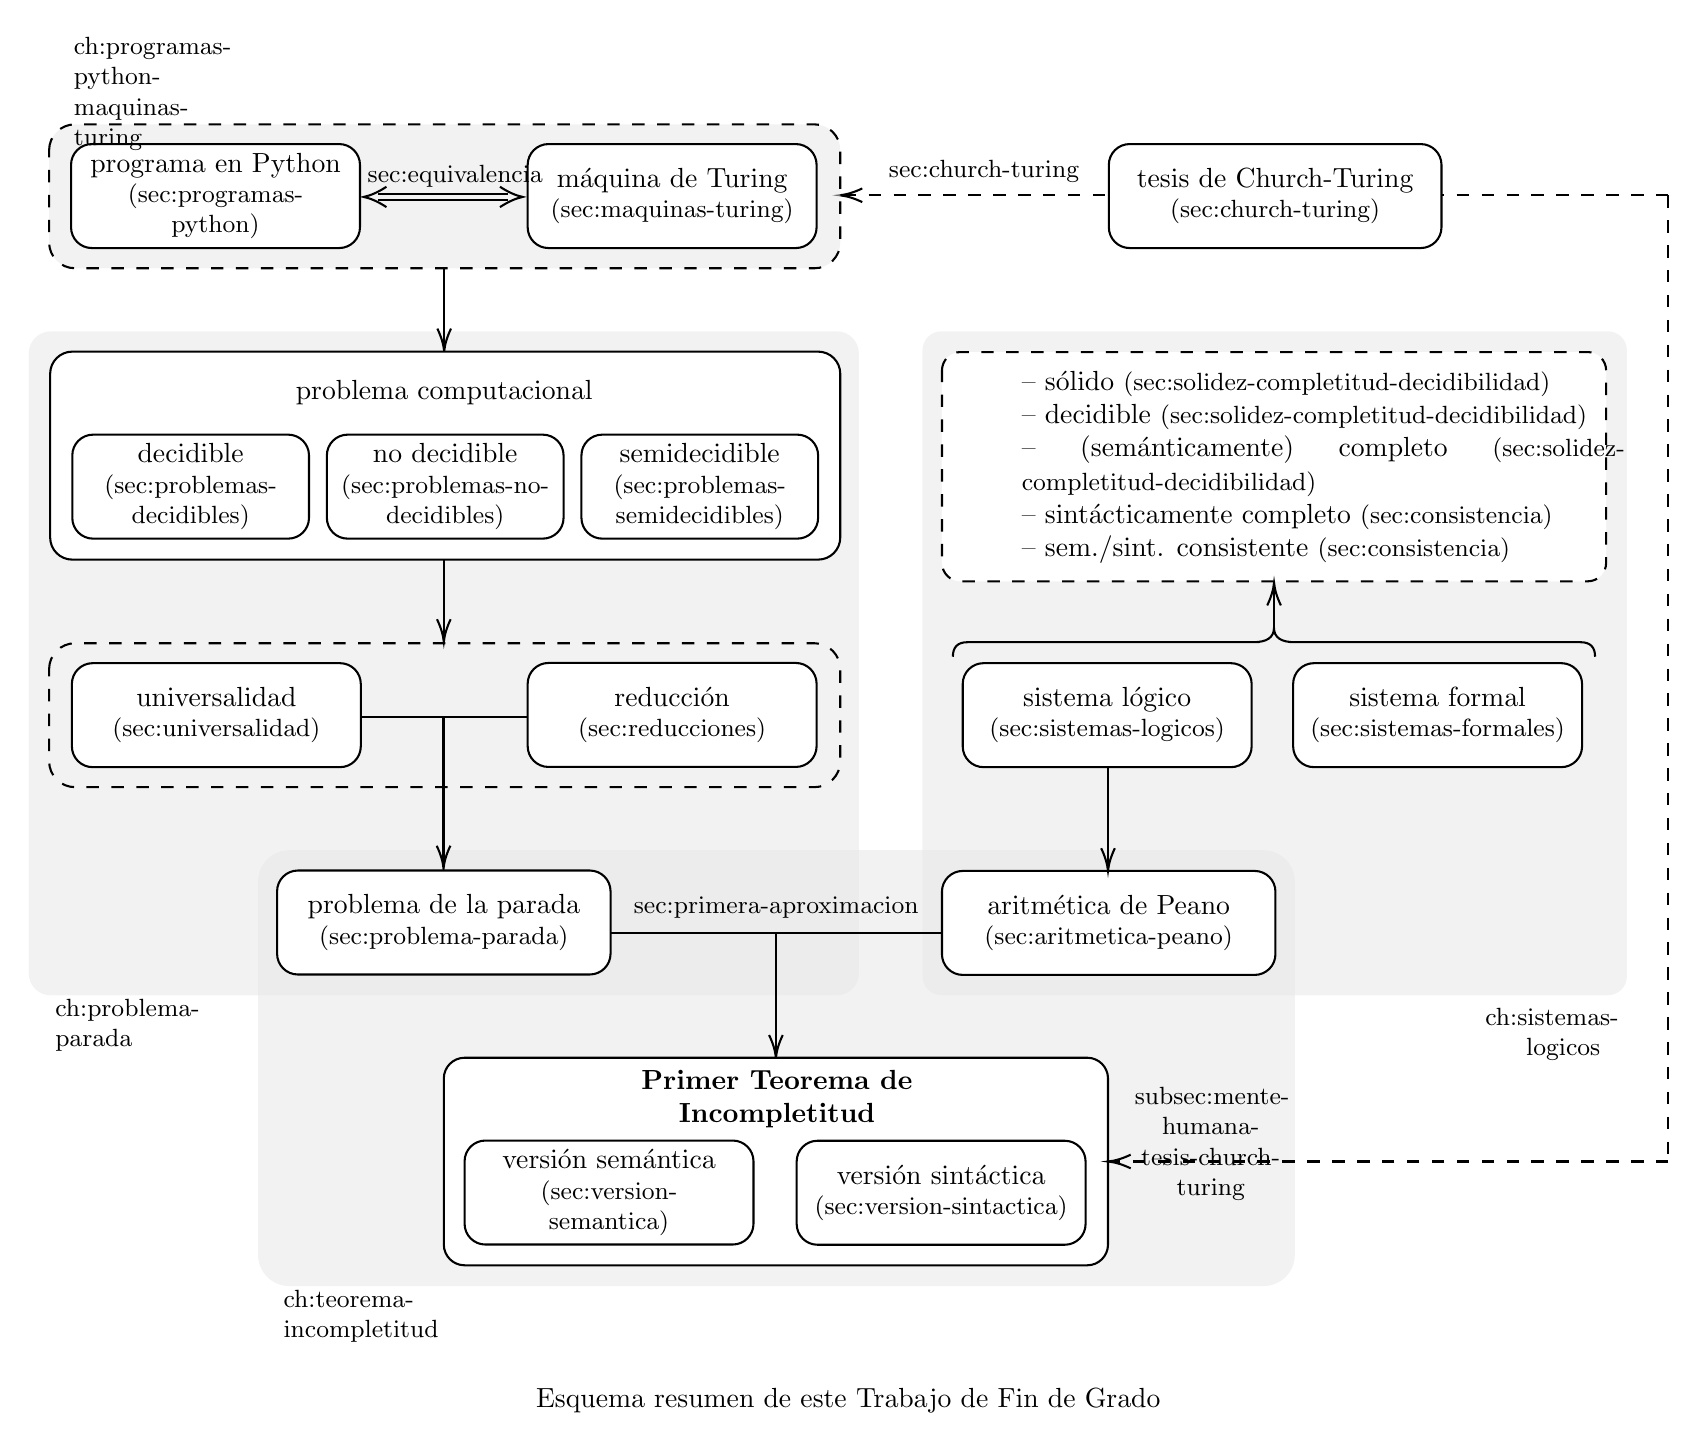
\begin{tikzpicture}[x=0.75pt,y=0.75pt,yscale=-1,xscale=1]
%uncomment if require: \path (0,694); %set diagram left start at 0, and has height of 694

%Straight Lines [id:da2056540562354816] 
\draw  [dash pattern={on 4.5pt off 4.5pt}]  (672,64.47) -- (810,64.47) ;
%Straight Lines [id:da23044041717189923] 
\draw  [dash pattern={on 4.5pt off 4.5pt}]  (412.67,64.47) -- (610,64.47) ;
\draw [shift={(410.67,64.47)}, rotate = 0] [color={rgb, 255:red, 0; green, 0; blue, 0 }  ][line width=0.75]    (10.93,-3.29) .. controls (6.95,-1.4) and (3.31,-0.3) .. (0,0) .. controls (3.31,0.3) and (6.95,1.4) .. (10.93,3.29)   ;
%Straight Lines [id:da8398435684999113] 
\draw  [dash pattern={on 4.5pt off 4.5pt}]  (810,64.47) -- (810,530) ;
%Rounded Rect [id:dp027018508739026448] 
\draw  [draw opacity=0][fill={rgb, 255:red, 230; green, 230; blue, 230 }  ,fill opacity=0.5 ] (20,439.33) .. controls (20,445.22) and (24.78,450) .. (30.67,450) -- (409.33,450) .. controls (415.22,450) and (420,445.22) .. (420,439.33) -- (420,140.67) .. controls (420,134.78) and (415.22,130) .. (409.33,130) -- (30.67,130) .. controls (24.78,130) and (20,134.78) .. (20,140.67) -- cycle ;
%Rounded Rect [id:dp9415679498487528] 
\draw  [dash pattern={on 4.5pt off 4.5pt}] (29.83,292.77) .. controls (29.83,285.88) and (35.41,280.3) .. (42.3,280.3) -- (398.54,280.3) .. controls (405.42,280.3) and (411,285.88) .. (411,292.77) -- (411,337.17) .. controls (411,344.05) and (405.42,349.64) .. (398.54,349.64) -- (42.3,349.64) .. controls (35.41,349.64) and (29.83,344.05) .. (29.83,337.17) -- cycle ;
%Rounded Rect [id:dp05100022295548956] 
\draw  [draw opacity=0][fill={rgb, 255:red, 230; green, 230; blue, 230 }  ,fill opacity=0.5 ] (130.5,575) .. controls (130.5,583.28) and (137.22,590) .. (145.5,590) -- (615,590) .. controls (623.28,590) and (630,583.28) .. (630,575) -- (630,395) .. controls (630,386.72) and (623.28,380) .. (615,380) -- (145.5,380) .. controls (137.22,380) and (130.5,386.72) .. (130.5,395) -- cycle ;
%Rounded Rect [id:dp6496809750851564] 
\draw  [draw opacity=0][fill={rgb, 255:red, 230; green, 230; blue, 230 }  ,fill opacity=0.5 ] (450.61,440.79) .. controls (450.61,445.82) and (454.69,449.9) .. (459.72,449.9) -- (780.89,449.9) .. controls (785.92,449.9) and (790,445.82) .. (790,440.79) -- (790,139.11) .. controls (790,134.08) and (785.92,130) .. (780.89,130) -- (459.72,130) .. controls (454.69,130) and (450.61,134.08) .. (450.61,139.11) -- cycle ;
%Rounded Rect [id:dp549636265291094] 
\draw  [fill={rgb, 255:red, 230; green, 230; blue, 230 }  ,fill opacity=0.5 ][dash pattern={on 4.5pt off 4.5pt}] (29.83,42.77) .. controls (29.83,35.88) and (35.41,30.3) .. (42.3,30.3) -- (398.54,30.3) .. controls (405.42,30.3) and (411,35.88) .. (411,42.77) -- (411,87.17) .. controls (411,94.05) and (405.42,99.64) .. (398.54,99.64) -- (42.3,99.64) .. controls (35.41,99.64) and (29.83,94.05) .. (29.83,87.17) -- cycle ;
%Rounded Rect [id:dp1378581119146769] 
\draw  [fill={rgb, 255:red, 255; green, 255; blue, 255 }  ,fill opacity=1 ] (40.4,49.82) .. controls (40.4,44.29) and (44.89,39.8) .. (50.42,39.8) -- (169.58,39.8) .. controls (175.11,39.8) and (179.6,44.29) .. (179.6,49.82) -- (179.6,79.88) .. controls (179.6,85.41) and (175.11,89.9) .. (169.58,89.9) -- (50.42,89.9) .. controls (44.89,89.9) and (40.4,85.41) .. (40.4,79.88) -- cycle ;
%Straight Lines [id:da8729153203483555] 
\draw    (188.42,63.77) -- (250.99,63.77)(188.42,66.77) -- (250.99,66.77) ;
\draw [shift={(257.99,65.27)}, rotate = 180] [color={rgb, 255:red, 0; green, 0; blue, 0 }  ][line width=0.75]    (10.93,-4.9) .. controls (6.95,-2.3) and (3.31,-0.67) .. (0,0) .. controls (3.31,0.67) and (6.95,2.3) .. (10.93,4.9)   ;
\draw [shift={(181.42,65.27)}, rotate = 0] [color={rgb, 255:red, 0; green, 0; blue, 0 }  ][line width=0.75]    (10.93,-4.9) .. controls (6.95,-2.3) and (3.31,-0.67) .. (0,0) .. controls (3.31,0.67) and (6.95,2.3) .. (10.93,4.9)   ;
%Straight Lines [id:da845243590120559] 
\draw    (220.17,99.97) -- (220.17,137.64) ;
\draw [shift={(220.17,139.64)}, rotate = 270] [color={rgb, 255:red, 0; green, 0; blue, 0 }  ][line width=0.75]    (10.93,-3.29) .. controls (6.95,-1.4) and (3.31,-0.3) .. (0,0) .. controls (3.31,0.3) and (6.95,1.4) .. (10.93,3.29)   ;
%Straight Lines [id:da7497001546502899] 
\draw    (380,420.33) -- (380,478) ;
\draw [shift={(380,480)}, rotate = 270] [color={rgb, 255:red, 0; green, 0; blue, 0 }  ][line width=0.75]    (10.93,-3.29) .. controls (6.95,-1.4) and (3.31,-0.3) .. (0,0) .. controls (3.31,0.3) and (6.95,1.4) .. (10.93,3.29)   ;
%Straight Lines [id:da5689893955334542] 
\draw    (300,420) -- (460,420) ;
%Rounded Rect [id:dp18582062333838767] 
\draw  [fill={rgb, 255:red, 255; green, 255; blue, 255 }  ,fill opacity=1 ] (260.4,49.82) .. controls (260.4,44.29) and (264.89,39.8) .. (270.42,39.8) -- (389.58,39.8) .. controls (395.11,39.8) and (399.6,44.29) .. (399.6,49.82) -- (399.6,79.88) .. controls (399.6,85.41) and (395.11,89.9) .. (389.58,89.9) -- (270.42,89.9) .. controls (264.89,89.9) and (260.4,85.41) .. (260.4,79.88) -- cycle ;
%Rounded Rect [id:dp9523169763067778] 
\draw  [fill={rgb, 255:red, 255; green, 255; blue, 255 }  ,fill opacity=1 ] (470,299.92) .. controls (470,294.39) and (474.49,289.9) .. (480.02,289.9) -- (599.18,289.9) .. controls (604.71,289.9) and (609.2,294.39) .. (609.2,299.92) -- (609.2,329.98) .. controls (609.2,335.51) and (604.71,340) .. (599.18,340) -- (480.02,340) .. controls (474.49,340) and (470,335.51) .. (470,329.98) -- cycle ;
%Rounded Rect [id:dp48544030815291705] 
\draw  [fill={rgb, 255:red, 255; green, 255; blue, 255 }  ,fill opacity=1 ] (220,490) .. controls (220,484.48) and (224.48,480) .. (230,480) -- (530,480) .. controls (535.52,480) and (540,484.48) .. (540,490) -- (540,570) .. controls (540,575.52) and (535.52,580) .. (530,580) -- (230,580) .. controls (224.48,580) and (220,575.52) .. (220,570) -- cycle ;
%Rounded Rect [id:dp08222627508455749] 
\draw  [fill={rgb, 255:red, 255; green, 255; blue, 255 }  ,fill opacity=1 ] (540.4,49.82) .. controls (540.4,44.29) and (544.89,39.8) .. (550.42,39.8) -- (690.65,39.8) .. controls (696.18,39.8) and (700.67,44.29) .. (700.67,49.82) -- (700.67,79.88) .. controls (700.67,85.41) and (696.18,89.9) .. (690.65,89.9) -- (550.42,89.9) .. controls (544.89,89.9) and (540.4,85.41) .. (540.4,79.88) -- cycle ;
%Straight Lines [id:da5868346364154593] 
\draw  [dash pattern={on 4.5pt off 4.5pt}]  (810,530) -- (542,530) ;
\draw [shift={(540,530)}, rotate = 360] [color={rgb, 255:red, 0; green, 0; blue, 0 }  ][line width=0.75]    (10.93,-3.29) .. controls (6.95,-1.4) and (3.31,-0.3) .. (0,0) .. controls (3.31,0.3) and (6.95,1.4) .. (10.93,3.29)   ;
%Rounded Rect [id:dp7392784471609453] 
\draw  [fill={rgb, 255:red, 255; green, 255; blue, 255 }  ,fill opacity=1 ] (30.33,150.47) .. controls (30.33,144.58) and (35.11,139.8) .. (41,139.8) -- (400.34,139.8) .. controls (406.23,139.8) and (411,144.58) .. (411,150.47) -- (411,229.34) .. controls (411,235.23) and (406.23,240.01) .. (400.34,240.01) -- (41,240.01) .. controls (35.11,240.01) and (30.33,235.23) .. (30.33,229.34) -- cycle ;
%Rounded Rect [id:dp90901637181607] 
\draw  [fill={rgb, 255:red, 255; green, 255; blue, 255 }  ,fill opacity=1 ] (41,189.82) .. controls (41,184.29) and (45.49,179.8) .. (51.02,179.8) -- (145.02,179.8) .. controls (150.55,179.8) and (155.04,184.29) .. (155.04,189.82) -- (155.04,219.88) .. controls (155.04,225.41) and (150.55,229.9) .. (145.02,229.9) -- (51.02,229.9) .. controls (45.49,229.9) and (41,225.41) .. (41,219.88) -- cycle ;
%Rounded Rect [id:dp06115018179625542] 
\draw  [fill={rgb, 255:red, 255; green, 255; blue, 255 }  ,fill opacity=1 ] (163.65,189.82) .. controls (163.65,184.29) and (168.13,179.8) .. (173.67,179.8) -- (267.67,179.8) .. controls (273.2,179.8) and (277.69,184.29) .. (277.69,189.82) -- (277.69,219.88) .. controls (277.69,225.41) and (273.2,229.9) .. (267.67,229.9) -- (173.67,229.9) .. controls (168.13,229.9) and (163.65,225.41) .. (163.65,219.88) -- cycle ;
%Rounded Rect [id:dp6195275548153432] 
\draw  [fill={rgb, 255:red, 255; green, 255; blue, 255 }  ,fill opacity=1 ] (286.3,189.82) .. controls (286.3,184.29) and (290.78,179.8) .. (296.32,179.8) -- (390.31,179.8) .. controls (395.85,179.8) and (400.33,184.29) .. (400.33,189.82) -- (400.33,219.88) .. controls (400.33,225.41) and (395.85,229.9) .. (390.31,229.9) -- (296.32,229.9) .. controls (290.78,229.9) and (286.3,225.41) .. (286.3,219.88) -- cycle ;
%Rounded Rect [id:dp41283415100159493] 
\draw  [fill={rgb, 255:red, 255; green, 255; blue, 255 }  ,fill opacity=1 ] (40.8,299.92) .. controls (40.8,294.39) and (45.29,289.9) .. (50.82,289.9) -- (169.98,289.9) .. controls (175.51,289.9) and (180,294.39) .. (180,299.92) -- (180,329.98) .. controls (180,335.51) and (175.51,340) .. (169.98,340) -- (50.82,340) .. controls (45.29,340) and (40.8,335.51) .. (40.8,329.98) -- cycle ;
%Rounded Rect [id:dp40154854661776396] 
\draw  [fill={rgb, 255:red, 255; green, 255; blue, 255 }  ,fill opacity=1 ] (260.4,299.82) .. controls (260.4,294.29) and (264.89,289.8) .. (270.42,289.8) -- (389.58,289.8) .. controls (395.11,289.8) and (399.6,294.29) .. (399.6,299.82) -- (399.6,329.88) .. controls (399.6,335.41) and (395.11,339.9) .. (389.58,339.9) -- (270.42,339.9) .. controls (264.89,339.9) and (260.4,335.41) .. (260.4,329.88) -- cycle ;
%Straight Lines [id:da6602630444249074] 
\draw    (180.17,315.8) -- (260,315.8) ;
%Straight Lines [id:da30905866347109745] 
\draw    (219.86,315.97) -- (219.86,386.81) ;
\draw [shift={(219.86,388.81)}, rotate = 270] [color={rgb, 255:red, 0; green, 0; blue, 0 }  ][line width=0.75]    (10.93,-3.29) .. controls (6.95,-1.4) and (3.31,-0.3) .. (0,0) .. controls (3.31,0.3) and (6.95,1.4) .. (10.93,3.29)   ;
%Rounded Rect [id:dp44627062039563214] 
\draw  [fill={rgb, 255:red, 255; green, 255; blue, 255 }  ,fill opacity=1 ] (139.67,399.82) .. controls (139.67,394.29) and (144.15,389.8) .. (149.69,389.8) -- (290.31,389.8) .. controls (295.85,389.8) and (300.33,394.29) .. (300.33,399.82) -- (300.33,429.88) .. controls (300.33,435.41) and (295.85,439.9) .. (290.31,439.9) -- (149.69,439.9) .. controls (144.15,439.9) and (139.67,435.41) .. (139.67,429.88) -- cycle ;
%Straight Lines [id:da8375870493480149] 
\draw    (220,240) -- (220,277.67) ;
\draw [shift={(220,279.67)}, rotate = 270] [color={rgb, 255:red, 0; green, 0; blue, 0 }  ][line width=0.75]    (10.93,-3.29) .. controls (6.95,-1.4) and (3.31,-0.3) .. (0,0) .. controls (3.31,0.3) and (6.95,1.4) .. (10.93,3.29)   ;
%Rounded Rect [id:dp37285624114093485] 
\draw  [fill={rgb, 255:red, 255; green, 255; blue, 255 }  ,fill opacity=1 ] (460,400.02) .. controls (460,394.49) and (464.49,390) .. (470.02,390) -- (610.65,390) .. controls (616.18,390) and (620.67,394.49) .. (620.67,400.02) -- (620.67,430.08) .. controls (620.67,435.61) and (616.18,440.1) .. (610.65,440.1) -- (470.02,440.1) .. controls (464.49,440.1) and (460,435.61) .. (460,430.08) -- cycle ;
%Rounded Rect [id:dp6883616335272991] 
\draw  [fill={rgb, 255:red, 255; green, 255; blue, 255 }  ,fill opacity=1 ] (629.2,299.92) .. controls (629.2,294.39) and (633.69,289.9) .. (639.22,289.9) -- (758.38,289.9) .. controls (763.91,289.9) and (768.4,294.39) .. (768.4,299.92) -- (768.4,329.98) .. controls (768.4,335.51) and (763.91,340) .. (758.38,340) -- (639.22,340) .. controls (633.69,340) and (629.2,335.51) .. (629.2,329.98) -- cycle ;
%Straight Lines [id:da19870419404011752] 
\draw    (540,340) -- (540,388) ;
\draw [shift={(540,390)}, rotate = 270] [color={rgb, 255:red, 0; green, 0; blue, 0 }  ][line width=0.75]    (10.93,-3.29) .. controls (6.95,-1.4) and (3.31,-0.3) .. (0,0) .. controls (3.31,0.3) and (6.95,1.4) .. (10.93,3.29)   ;
%Rounded Rect [id:dp9692784599420237] 
\draw  [fill={rgb, 255:red, 255; green, 255; blue, 255 }  ,fill opacity=1 ] (230,529.92) .. controls (230,524.39) and (234.49,519.9) .. (240.02,519.9) -- (359.18,519.9) .. controls (364.71,519.9) and (369.2,524.39) .. (369.2,529.92) -- (369.2,559.98) .. controls (369.2,565.51) and (364.71,570) .. (359.18,570) -- (240.02,570) .. controls (234.49,570) and (230,565.51) .. (230,559.98) -- cycle ;
%Rounded Rect [id:dp749684165723072] 
\draw  [fill={rgb, 255:red, 255; green, 255; blue, 255 }  ,fill opacity=1 ] (390,530.02) .. controls (390,524.49) and (394.49,520) .. (400.02,520) -- (519.18,520) .. controls (524.71,520) and (529.2,524.49) .. (529.2,530.02) -- (529.2,560.08) .. controls (529.2,565.61) and (524.71,570.1) .. (519.18,570.1) -- (400.02,570.1) .. controls (394.49,570.1) and (390,565.61) .. (390,560.08) -- cycle ;
%Rounded Rect [id:dp28001422897762485] 
\draw  [fill={rgb, 255:red, 255; green, 255; blue, 255 }  ,fill opacity=1 ][dash pattern={on 4.5pt off 4.5pt}] (460,148.92) .. controls (460,143.99) and (463.99,140) .. (468.92,140) -- (771.08,140) .. controls (776.01,140) and (780,143.99) .. (780,148.92) -- (780,241.55) .. controls (780,246.48) and (776.01,250.47) .. (771.08,250.47) -- (468.92,250.47) .. controls (463.99,250.47) and (460,246.48) .. (460,241.55) -- cycle ;
%Shape: Brace [id:dp9411387904179627] 
\draw   (774.67,286.8) .. controls (774.67,282.13) and (772.34,279.8) .. (767.67,279.8) -- (629.96,279.8) .. controls (623.29,279.8) and (619.96,277.47) .. (619.96,272.8) .. controls (619.96,277.47) and (616.63,279.8) .. (609.96,279.8)(612.96,279.8) -- (472.25,279.8) .. controls (467.58,279.8) and (465.25,282.13) .. (465.25,286.8) ;
%Straight Lines [id:da9902399507274253] 
\draw    (620,273) -- (620,253.14) ;
\draw [shift={(620,251.14)}, rotate = 90] [color={rgb, 255:red, 0; green, 0; blue, 0 }  ][line width=0.75]    (10.93,-3.29) .. controls (6.95,-1.4) and (3.31,-0.3) .. (0,0) .. controls (3.31,0.3) and (6.95,1.4) .. (10.93,3.29)   ;

% Text Node
\draw (110,64.85) node  [color={rgb, 255:red, 0; green, 0; blue, 0 }  ,opacity=1 ] [align=left] {\begin{minipage}[lt]{92.93pt}\setlength\topsep{0pt}
\begin{center}
programa en Python\\
\small{(\cref{sec:programas-python})}
\end{center}

\end{minipage}};
% Text Node
\draw (219.89,51.97) node  [font=\small,color={rgb, 255:red, 0; green, 0; blue, 0 }  ,opacity=1 ] [align=left] {\begin{minipage}[lt]{54.86pt}\setlength\topsep{0pt}
\begin{center}
\Cref{sec:equivalencia}
\end{center}

\end{minipage}};
% Text Node
\draw (69.5,15.5) node  [font=\small,color={rgb, 255:red, 0; green, 0; blue, 0 }  ,opacity=1 ] [align=left] {\begin{minipage}[lt]{41.55pt}\setlength\topsep{0pt}
\cref{ch:programas-python-maquinas-turing}
\end{minipage}};
% Text Node
\draw (330,64.85) node  [color={rgb, 255:red, 0; green, 0; blue, 0 }  ,opacity=1 ] [align=left] {\begin{minipage}[lt]{92.93pt}\setlength\topsep{0pt}
\begin{center}
máquina de Turing\\
\small{(\cref{sec:maquinas-turing})}
\end{center}

\end{minipage}};
% Text Node
\draw (539.6,314.95) node  [color={rgb, 255:red, 0; green, 0; blue, 0 }  ,opacity=1 ] [align=left] {\begin{minipage}[lt]{92.93pt}\setlength\topsep{0pt}
\begin{center}
sistema lógico\\
\small{(\cref{sec:sistemas-logicos})}
\end{center}

\end{minipage}};
% Text Node
\draw (380.5,500.11) node  [color={rgb, 255:red, 0; green, 0; blue, 0 }  ,opacity=1 ] [align=left] {\begin{minipage}[lt]{159.55pt}\setlength\topsep{0pt}
\begin{center}
\textbf{Primer Teorema de Incompletitud}
\end{center}

\end{minipage}};
% Text Node
\draw (620.53,64.85) node  [color={rgb, 255:red, 0; green, 0; blue, 0 }  ,opacity=1 ] [align=left] {\begin{minipage}[lt]{106.99pt}\setlength\topsep{0pt}
\begin{center}
tesis de Church-Turing\\
\small{(\cref{sec:church-turing})}
\end{center}

\end{minipage}};
% Text Node
\draw (480.28,52.8) node  [font=\small,color={rgb, 255:red, 0; green, 0; blue, 0 }  ,opacity=1 ] [align=left] {\begin{minipage}[lt]{81.9pt}\setlength\topsep{0pt}
\begin{center}
\cref{sec:church-turing}
\end{center}

\end{minipage}};
% Text Node
\draw (589.5,518.3) node  [font=\small,color={rgb, 255:red, 0; green, 0; blue, 0 }  ,opacity=1 ] [align=left] {\begin{minipage}[lt]{54.86pt}\setlength\topsep{0pt}
\begin{center}
\Cref{subsec:mente-humana-tesis-church-turing}
\end{center}

\end{minipage}};
% Text Node
\draw (220.2,159.62) node  [color={rgb, 255:red, 0; green, 0; blue, 0 }  ,opacity=1 ] [align=left] {\begin{minipage}[lt]{230.11pt}\setlength\topsep{0pt}
\begin{center}
problema computacional
\end{center}

\end{minipage}};
% Text Node
\draw (98.02,204.85) node  [color={rgb, 255:red, 0; green, 0; blue, 0 }  ,opacity=1 ] [align=left] {\begin{minipage}[lt]{76.13pt}\setlength\topsep{0pt}
\begin{center}
decidible\\
\small{(\cref{sec:problemas-decidibles})}
\end{center}

\end{minipage}};
% Text Node
\draw (220.67,204.85) node  [color={rgb, 255:red, 0; green, 0; blue, 0 }  ,opacity=1 ] [align=left] {\begin{minipage}[lt]{76.13pt}\setlength\topsep{0pt}
\begin{center}
no decidible\\
\small{(\cref{sec:problemas-no-decidibles})}
\end{center}

\end{minipage}};
% Text Node
\draw (343.31,204.85) node  [color={rgb, 255:red, 0; green, 0; blue, 0 }  ,opacity=1 ] [align=left] {\begin{minipage}[lt]{76.13pt}\setlength\topsep{0pt}
\begin{center}
semidecidible\\
\small{(\cref{sec:problemas-semidecidibles})}
\end{center}

\end{minipage}};
% Text Node
\draw (110.4,314.95) node  [color={rgb, 255:red, 0; green, 0; blue, 0 }  ,opacity=1 ] [align=left] {\begin{minipage}[lt]{92.93pt}\setlength\topsep{0pt}
\begin{center}
universalidad\\
\small{(\cref{sec:universalidad})}
\end{center}

\end{minipage}};
% Text Node
\draw (330,314.85) node  [color={rgb, 255:red, 0; green, 0; blue, 0 }  ,opacity=1 ] [align=left] {\begin{minipage}[lt]{92.93pt}\setlength\topsep{0pt}
\begin{center}
reducción\\
\small{(\cref{sec:reducciones})}
\end{center}

\end{minipage}};
% Text Node
\draw (220,414.85) node  [color={rgb, 255:red, 0; green, 0; blue, 0 }  ,opacity=1 ] [align=left] {\begin{minipage}[lt]{107.26pt}\setlength\topsep{0pt}
\begin{center}
problema de la parada\\
\small{(\cref{sec:problema-parada})}
\end{center}

\end{minipage}};
% Text Node
\draw (540.33,415.05) node  [color={rgb, 255:red, 0; green, 0; blue, 0 }  ,opacity=1 ] [align=left] {\begin{minipage}[lt]{107.26pt}\setlength\topsep{0pt}
\begin{center}
aritmética de Peano\\
\small{(\cref{sec:aritmetica-peano})}
\end{center}

\end{minipage}};
% Text Node
\draw (698.8,314.95) node  [color={rgb, 255:red, 0; green, 0; blue, 0 }  ,opacity=1 ] [align=left] {\begin{minipage}[lt]{92.93pt}\setlength\topsep{0pt}
\begin{center}
sistema formal\\
\small{(\cref{sec:sistemas-formales})}
\end{center}

\end{minipage}};
% Text Node
\draw (299.6,544.95) node  [color={rgb, 255:red, 0; green, 0; blue, 0 }  ,opacity=1 ] [align=left] {\begin{minipage}[lt]{92.93pt}\setlength\topsep{0pt}
\begin{center}
versión semántica\\
\small{(\cref{sec:version-semantica})}
\end{center}

\end{minipage}};
% Text Node
\draw (459.6,545.05) node  [color={rgb, 255:red, 0; green, 0; blue, 0 }  ,opacity=1 ] [align=left] {\begin{minipage}[lt]{92.93pt}\setlength\topsep{0pt}
\begin{center}
versión sintáctica\\
\small{(\cref{sec:version-sintactica})}
\end{center}

\end{minipage}};
% Text Node
\draw (60.5,464.5) node  [font=\small,color={rgb, 255:red, 0; green, 0; blue, 0 }  ,opacity=1 ] [align=left] {\begin{minipage}[lt]{41.55pt}\setlength\topsep{0pt}
\cref{ch:problema-parada}
\end{minipage}};
% Text Node
\draw (749.5,465.5) node  [font=\small,color={rgb, 255:red, 0; green, 0; blue, 0 }  ,opacity=1 ] [align=left] {\begin{minipage}[lt]{41.55pt}\setlength\topsep{0pt}
\begin{flushright}
\cref{ch:sistemas-logicos}
\end{flushright}

\end{minipage}};
% Text Node
\draw (170.5,604.5) node  [font=\small,color={rgb, 255:red, 0; green, 0; blue, 0 }  ,opacity=1 ] [align=left] {\begin{minipage}[lt]{41.55pt}\setlength\topsep{0pt}
\cref{ch:teorema-incompletitud}
\end{minipage}};
% Text Node
\draw (643.76,195.55) node  [color={rgb, 255:red, 0; green, 0; blue, 0 }  ,opacity=1 ] [align=left] {\begin{minipage}[lt]{217.92pt}\setlength\topsep{0pt}
-- sólido {\small{(\cref{sec:solidez-completitud-decidibilidad})}}\\
-- decidible {\small{(\cref{sec:solidez-completitud-decidibilidad})}}\\
-- (semánticamente) completo {\small{(\cref{sec:solidez-completitud-decidibilidad})}}\\
-- sintácticamente completo {\small{(\cref{sec:consistencia})}}\\
-- sem./sint. consistente {\small{(\cref{sec:consistencia})}}
\end{minipage}};
% Text Node
\draw (414.84,645.25) node  [color={rgb, 255:red, 0; green, 0; blue, 0 }  ,opacity=1 ] [align=left] {\begin{minipage}[lt]{534.7pt}\setlength\topsep{0pt}
\begin{center}
Esquema resumen de este Trabajo de Fin de Grado
\end{center}
\end{minipage}};
% Text Node
\draw (380.15,407.8) node  [font=\small,color={rgb, 255:red, 0; green, 0; blue, 0 }  ,opacity=1 ] [align=left] {\begin{minipage}[lt]{108.93pt}\setlength\topsep{0pt}
\begin{center}
\cref{sec:primera-aproximacion}
\end{center}

\end{minipage}};

\end{tikzpicture}
%\raisebox{-15.5cm}[0pt][0pt]{%
%\resizebox{\linewidth}{!}{

\tikzset{every picture/.style={line width=0.75pt}} %set default line width to 0.75pt        

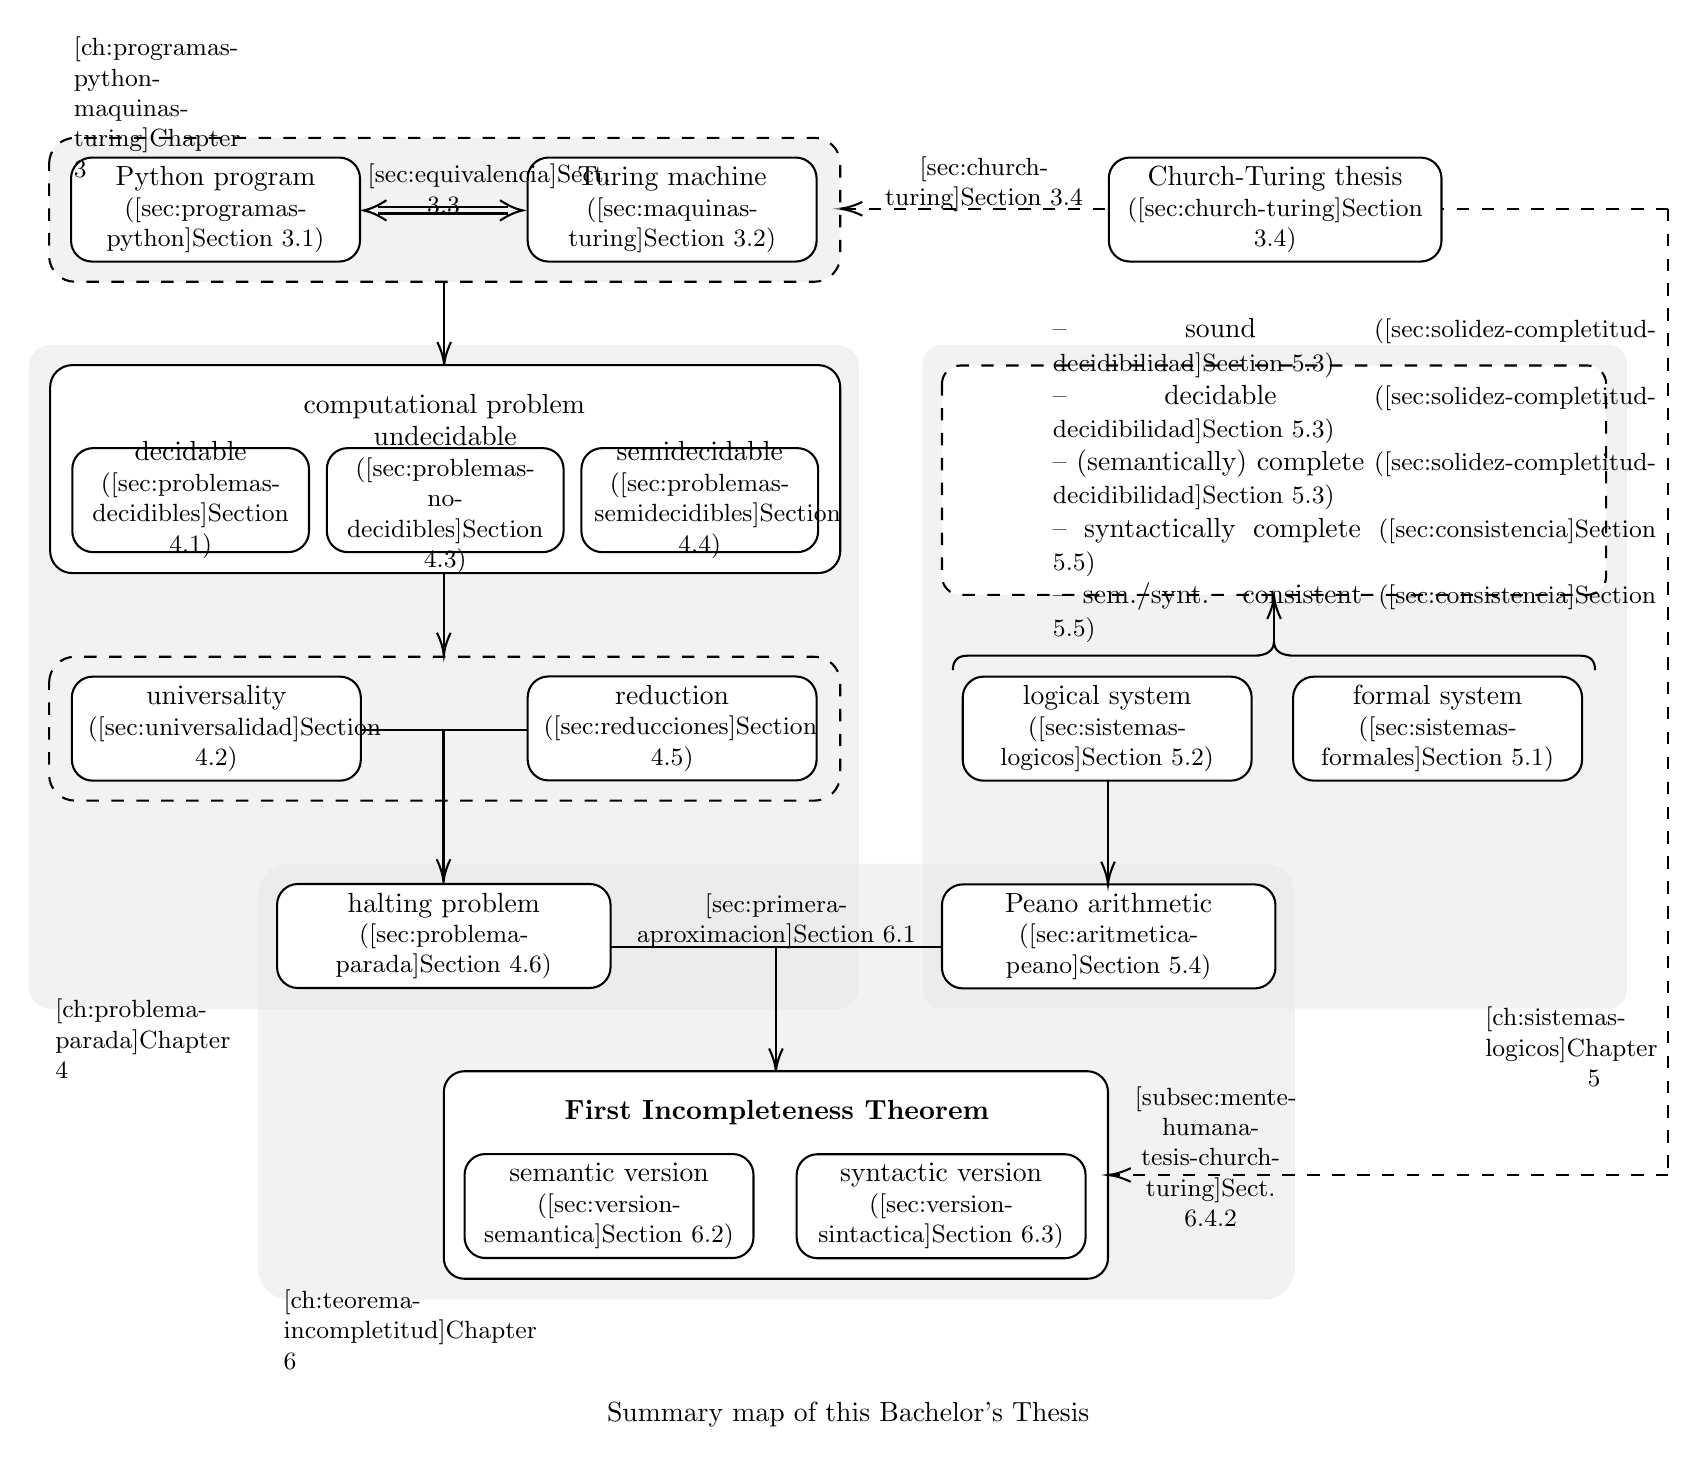
\begin{tikzpicture}[x=0.75pt,y=0.75pt,yscale=-1,xscale=1]
%uncomment if require: \path (0,694); %set diagram left start at 0, and has height of 694

%Straight Lines [id:da2056540562354816] 
\draw  [dash pattern={on 4.5pt off 4.5pt}]  (672,64.47) -- (810,64.47) ;
%Straight Lines [id:da23044041717189923] 
\draw  [dash pattern={on 4.5pt off 4.5pt}]  (412.67,64.47) -- (610,64.47) ;
\draw [shift={(410.67,64.47)}, rotate = 0] [color={rgb, 255:red, 0; green, 0; blue, 0 }  ][line width=0.75]    (10.93,-3.29) .. controls (6.95,-1.4) and (3.31,-0.3) .. (0,0) .. controls (3.31,0.3) and (6.95,1.4) .. (10.93,3.29)   ;
%Straight Lines [id:da8398435684999113] 
\draw  [dash pattern={on 4.5pt off 4.5pt}]  (810,64.47) -- (810,530) ;
%Rounded Rect [id:dp027018508739026448] 
\draw  [draw opacity=0][fill={rgb, 255:red, 230; green, 230; blue, 230 }  ,fill opacity=0.5 ] (20,439.33) .. controls (20,445.22) and (24.78,450) .. (30.67,450) -- (409.33,450) .. controls (415.22,450) and (420,445.22) .. (420,439.33) -- (420,140.67) .. controls (420,134.78) and (415.22,130) .. (409.33,130) -- (30.67,130) .. controls (24.78,130) and (20,134.78) .. (20,140.67) -- cycle ;
%Rounded Rect [id:dp9415679498487528] 
\draw  [dash pattern={on 4.5pt off 4.5pt}] (29.83,292.77) .. controls (29.83,285.88) and (35.41,280.3) .. (42.3,280.3) -- (398.54,280.3) .. controls (405.42,280.3) and (411,285.88) .. (411,292.77) -- (411,337.17) .. controls (411,344.05) and (405.42,349.64) .. (398.54,349.64) -- (42.3,349.64) .. controls (35.41,349.64) and (29.83,344.05) .. (29.83,337.17) -- cycle ;
%Rounded Rect [id:dp05100022295548956] 
\draw  [draw opacity=0][fill={rgb, 255:red, 230; green, 230; blue, 230 }  ,fill opacity=0.5 ] (130.5,575) .. controls (130.5,583.28) and (137.22,590) .. (145.5,590) -- (615,590) .. controls (623.28,590) and (630,583.28) .. (630,575) -- (630,395) .. controls (630,386.72) and (623.28,380) .. (615,380) -- (145.5,380) .. controls (137.22,380) and (130.5,386.72) .. (130.5,395) -- cycle ;
%Rounded Rect [id:dp6496809750851564] 
\draw  [draw opacity=0][fill={rgb, 255:red, 230; green, 230; blue, 230 }  ,fill opacity=0.5 ] (450.61,440.79) .. controls (450.61,445.82) and (454.69,449.9) .. (459.72,449.9) -- (780.89,449.9) .. controls (785.92,449.9) and (790,445.82) .. (790,440.79) -- (790,139.11) .. controls (790,134.08) and (785.92,130) .. (780.89,130) -- (459.72,130) .. controls (454.69,130) and (450.61,134.08) .. (450.61,139.11) -- cycle ;
%Rounded Rect [id:dp549636265291094] 
\draw  [fill={rgb, 255:red, 230; green, 230; blue, 230 }  ,fill opacity=0.5 ][dash pattern={on 4.5pt off 4.5pt}] (29.83,42.77) .. controls (29.83,35.88) and (35.41,30.3) .. (42.3,30.3) -- (398.54,30.3) .. controls (405.42,30.3) and (411,35.88) .. (411,42.77) -- (411,87.17) .. controls (411,94.05) and (405.42,99.64) .. (398.54,99.64) -- (42.3,99.64) .. controls (35.41,99.64) and (29.83,94.05) .. (29.83,87.17) -- cycle ;
%Rounded Rect [id:dp1378581119146769] 
\draw  [fill={rgb, 255:red, 255; green, 255; blue, 255 }  ,fill opacity=1 ] (40.4,49.82) .. controls (40.4,44.29) and (44.89,39.8) .. (50.42,39.8) -- (169.58,39.8) .. controls (175.11,39.8) and (179.6,44.29) .. (179.6,49.82) -- (179.6,79.88) .. controls (179.6,85.41) and (175.11,89.9) .. (169.58,89.9) -- (50.42,89.9) .. controls (44.89,89.9) and (40.4,85.41) .. (40.4,79.88) -- cycle ;
%Straight Lines [id:da8729153203483555] 
\draw    (188.42,63.77) -- (250.99,63.77)(188.42,66.77) -- (250.99,66.77) ;
\draw [shift={(257.99,65.27)}, rotate = 180] [color={rgb, 255:red, 0; green, 0; blue, 0 }  ][line width=0.75]    (10.93,-4.9) .. controls (6.95,-2.3) and (3.31,-0.67) .. (0,0) .. controls (3.31,0.67) and (6.95,2.3) .. (10.93,4.9)   ;
\draw [shift={(181.42,65.27)}, rotate = 0] [color={rgb, 255:red, 0; green, 0; blue, 0 }  ][line width=0.75]    (10.93,-4.9) .. controls (6.95,-2.3) and (3.31,-0.67) .. (0,0) .. controls (3.31,0.67) and (6.95,2.3) .. (10.93,4.9)   ;
%Straight Lines [id:da845243590120559] 
\draw    (220.17,99.97) -- (220.17,137.64) ;
\draw [shift={(220.17,139.64)}, rotate = 270] [color={rgb, 255:red, 0; green, 0; blue, 0 }  ][line width=0.75]    (10.93,-3.29) .. controls (6.95,-1.4) and (3.31,-0.3) .. (0,0) .. controls (3.31,0.3) and (6.95,1.4) .. (10.93,3.29)   ;
%Straight Lines [id:da7497001546502899] 
\draw    (380,420.33) -- (380,478) ;
\draw [shift={(380,480)}, rotate = 270] [color={rgb, 255:red, 0; green, 0; blue, 0 }  ][line width=0.75]    (10.93,-3.29) .. controls (6.95,-1.4) and (3.31,-0.3) .. (0,0) .. controls (3.31,0.3) and (6.95,1.4) .. (10.93,3.29)   ;
%Straight Lines [id:da5689893955334542] 
\draw    (300,420) -- (460,420) ;
%Rounded Rect [id:dp18582062333838767] 
\draw  [fill={rgb, 255:red, 255; green, 255; blue, 255 }  ,fill opacity=1 ] (260.4,49.82) .. controls (260.4,44.29) and (264.89,39.8) .. (270.42,39.8) -- (389.58,39.8) .. controls (395.11,39.8) and (399.6,44.29) .. (399.6,49.82) -- (399.6,79.88) .. controls (399.6,85.41) and (395.11,89.9) .. (389.58,89.9) -- (270.42,89.9) .. controls (264.89,89.9) and (260.4,85.41) .. (260.4,79.88) -- cycle ;
%Rounded Rect [id:dp9523169763067778] 
\draw  [fill={rgb, 255:red, 255; green, 255; blue, 255 }  ,fill opacity=1 ] (470,299.92) .. controls (470,294.39) and (474.49,289.9) .. (480.02,289.9) -- (599.18,289.9) .. controls (604.71,289.9) and (609.2,294.39) .. (609.2,299.92) -- (609.2,329.98) .. controls (609.2,335.51) and (604.71,340) .. (599.18,340) -- (480.02,340) .. controls (474.49,340) and (470,335.51) .. (470,329.98) -- cycle ;
%Rounded Rect [id:dp48544030815291705] 
\draw  [fill={rgb, 255:red, 255; green, 255; blue, 255 }  ,fill opacity=1 ] (220,490) .. controls (220,484.48) and (224.48,480) .. (230,480) -- (530,480) .. controls (535.52,480) and (540,484.48) .. (540,490) -- (540,570) .. controls (540,575.52) and (535.52,580) .. (530,580) -- (230,580) .. controls (224.48,580) and (220,575.52) .. (220,570) -- cycle ;
%Rounded Rect [id:dp08222627508455749] 
\draw  [fill={rgb, 255:red, 255; green, 255; blue, 255 }  ,fill opacity=1 ] (540.4,49.82) .. controls (540.4,44.29) and (544.89,39.8) .. (550.42,39.8) -- (690.65,39.8) .. controls (696.18,39.8) and (700.67,44.29) .. (700.67,49.82) -- (700.67,79.88) .. controls (700.67,85.41) and (696.18,89.9) .. (690.65,89.9) -- (550.42,89.9) .. controls (544.89,89.9) and (540.4,85.41) .. (540.4,79.88) -- cycle ;
%Straight Lines [id:da5868346364154593] 
\draw  [dash pattern={on 4.5pt off 4.5pt}]  (810,530) -- (542,530) ;
\draw [shift={(540,530)}, rotate = 360] [color={rgb, 255:red, 0; green, 0; blue, 0 }  ][line width=0.75]    (10.93,-3.29) .. controls (6.95,-1.4) and (3.31,-0.3) .. (0,0) .. controls (3.31,0.3) and (6.95,1.4) .. (10.93,3.29)   ;
%Rounded Rect [id:dp7392784471609453] 
\draw  [fill={rgb, 255:red, 255; green, 255; blue, 255 }  ,fill opacity=1 ] (30.33,150.47) .. controls (30.33,144.58) and (35.11,139.8) .. (41,139.8) -- (400.34,139.8) .. controls (406.23,139.8) and (411,144.58) .. (411,150.47) -- (411,229.34) .. controls (411,235.23) and (406.23,240.01) .. (400.34,240.01) -- (41,240.01) .. controls (35.11,240.01) and (30.33,235.23) .. (30.33,229.34) -- cycle ;
%Rounded Rect [id:dp90901637181607] 
\draw  [fill={rgb, 255:red, 255; green, 255; blue, 255 }  ,fill opacity=1 ] (41,189.82) .. controls (41,184.29) and (45.49,179.8) .. (51.02,179.8) -- (145.02,179.8) .. controls (150.55,179.8) and (155.04,184.29) .. (155.04,189.82) -- (155.04,219.88) .. controls (155.04,225.41) and (150.55,229.9) .. (145.02,229.9) -- (51.02,229.9) .. controls (45.49,229.9) and (41,225.41) .. (41,219.88) -- cycle ;
%Rounded Rect [id:dp06115018179625542] 
\draw  [fill={rgb, 255:red, 255; green, 255; blue, 255 }  ,fill opacity=1 ] (163.65,189.82) .. controls (163.65,184.29) and (168.13,179.8) .. (173.67,179.8) -- (267.67,179.8) .. controls (273.2,179.8) and (277.69,184.29) .. (277.69,189.82) -- (277.69,219.88) .. controls (277.69,225.41) and (273.2,229.9) .. (267.67,229.9) -- (173.67,229.9) .. controls (168.13,229.9) and (163.65,225.41) .. (163.65,219.88) -- cycle ;
%Rounded Rect [id:dp6195275548153432] 
\draw  [fill={rgb, 255:red, 255; green, 255; blue, 255 }  ,fill opacity=1 ] (286.3,189.82) .. controls (286.3,184.29) and (290.78,179.8) .. (296.32,179.8) -- (390.31,179.8) .. controls (395.85,179.8) and (400.33,184.29) .. (400.33,189.82) -- (400.33,219.88) .. controls (400.33,225.41) and (395.85,229.9) .. (390.31,229.9) -- (296.32,229.9) .. controls (290.78,229.9) and (286.3,225.41) .. (286.3,219.88) -- cycle ;
%Rounded Rect [id:dp41283415100159493] 
\draw  [fill={rgb, 255:red, 255; green, 255; blue, 255 }  ,fill opacity=1 ] (40.8,299.92) .. controls (40.8,294.39) and (45.29,289.9) .. (50.82,289.9) -- (169.98,289.9) .. controls (175.51,289.9) and (180,294.39) .. (180,299.92) -- (180,329.98) .. controls (180,335.51) and (175.51,340) .. (169.98,340) -- (50.82,340) .. controls (45.29,340) and (40.8,335.51) .. (40.8,329.98) -- cycle ;
%Rounded Rect [id:dp40154854661776396] 
\draw  [fill={rgb, 255:red, 255; green, 255; blue, 255 }  ,fill opacity=1 ] (260.4,299.82) .. controls (260.4,294.29) and (264.89,289.8) .. (270.42,289.8) -- (389.58,289.8) .. controls (395.11,289.8) and (399.6,294.29) .. (399.6,299.82) -- (399.6,329.88) .. controls (399.6,335.41) and (395.11,339.9) .. (389.58,339.9) -- (270.42,339.9) .. controls (264.89,339.9) and (260.4,335.41) .. (260.4,329.88) -- cycle ;
%Straight Lines [id:da6602630444249074] 
\draw    (180.17,315.8) -- (260,315.8) ;
%Straight Lines [id:da30905866347109745] 
\draw    (219.86,315.97) -- (219.86,386.81) ;
\draw [shift={(219.86,388.81)}, rotate = 270] [color={rgb, 255:red, 0; green, 0; blue, 0 }  ][line width=0.75]    (10.93,-3.29) .. controls (6.95,-1.4) and (3.31,-0.3) .. (0,0) .. controls (3.31,0.3) and (6.95,1.4) .. (10.93,3.29)   ;
%Rounded Rect [id:dp44627062039563214] 
\draw  [fill={rgb, 255:red, 255; green, 255; blue, 255 }  ,fill opacity=1 ] (139.67,399.82) .. controls (139.67,394.29) and (144.15,389.8) .. (149.69,389.8) -- (290.31,389.8) .. controls (295.85,389.8) and (300.33,394.29) .. (300.33,399.82) -- (300.33,429.88) .. controls (300.33,435.41) and (295.85,439.9) .. (290.31,439.9) -- (149.69,439.9) .. controls (144.15,439.9) and (139.67,435.41) .. (139.67,429.88) -- cycle ;
%Straight Lines [id:da8375870493480149] 
\draw    (220,240) -- (220,277.67) ;
\draw [shift={(220,279.67)}, rotate = 270] [color={rgb, 255:red, 0; green, 0; blue, 0 }  ][line width=0.75]    (10.93,-3.29) .. controls (6.95,-1.4) and (3.31,-0.3) .. (0,0) .. controls (3.31,0.3) and (6.95,1.4) .. (10.93,3.29)   ;
%Rounded Rect [id:dp37285624114093485] 
\draw  [fill={rgb, 255:red, 255; green, 255; blue, 255 }  ,fill opacity=1 ] (460,400.02) .. controls (460,394.49) and (464.49,390) .. (470.02,390) -- (610.65,390) .. controls (616.18,390) and (620.67,394.49) .. (620.67,400.02) -- (620.67,430.08) .. controls (620.67,435.61) and (616.18,440.1) .. (610.65,440.1) -- (470.02,440.1) .. controls (464.49,440.1) and (460,435.61) .. (460,430.08) -- cycle ;
%Rounded Rect [id:dp6883616335272991] 
\draw  [fill={rgb, 255:red, 255; green, 255; blue, 255 }  ,fill opacity=1 ] (629.2,299.92) .. controls (629.2,294.39) and (633.69,289.9) .. (639.22,289.9) -- (758.38,289.9) .. controls (763.91,289.9) and (768.4,294.39) .. (768.4,299.92) -- (768.4,329.98) .. controls (768.4,335.51) and (763.91,340) .. (758.38,340) -- (639.22,340) .. controls (633.69,340) and (629.2,335.51) .. (629.2,329.98) -- cycle ;
%Straight Lines [id:da19870419404011752] 
\draw    (540,340) -- (540,388) ;
\draw [shift={(540,390)}, rotate = 270] [color={rgb, 255:red, 0; green, 0; blue, 0 }  ][line width=0.75]    (10.93,-3.29) .. controls (6.95,-1.4) and (3.31,-0.3) .. (0,0) .. controls (3.31,0.3) and (6.95,1.4) .. (10.93,3.29)   ;
%Rounded Rect [id:dp9692784599420237] 
\draw  [fill={rgb, 255:red, 255; green, 255; blue, 255 }  ,fill opacity=1 ] (230,529.92) .. controls (230,524.39) and (234.49,519.9) .. (240.02,519.9) -- (359.18,519.9) .. controls (364.71,519.9) and (369.2,524.39) .. (369.2,529.92) -- (369.2,559.98) .. controls (369.2,565.51) and (364.71,570) .. (359.18,570) -- (240.02,570) .. controls (234.49,570) and (230,565.51) .. (230,559.98) -- cycle ;
%Rounded Rect [id:dp749684165723072] 
\draw  [fill={rgb, 255:red, 255; green, 255; blue, 255 }  ,fill opacity=1 ] (390,530.02) .. controls (390,524.49) and (394.49,520) .. (400.02,520) -- (519.18,520) .. controls (524.71,520) and (529.2,524.49) .. (529.2,530.02) -- (529.2,560.08) .. controls (529.2,565.61) and (524.71,570.1) .. (519.18,570.1) -- (400.02,570.1) .. controls (394.49,570.1) and (390,565.61) .. (390,560.08) -- cycle ;
%Rounded Rect [id:dp28001422897762485] 
\draw  [fill={rgb, 255:red, 255; green, 255; blue, 255 }  ,fill opacity=1 ][dash pattern={on 4.5pt off 4.5pt}] (460,148.92) .. controls (460,143.99) and (463.99,140) .. (468.92,140) -- (771.08,140) .. controls (776.01,140) and (780,143.99) .. (780,148.92) -- (780,241.55) .. controls (780,246.48) and (776.01,250.47) .. (771.08,250.47) -- (468.92,250.47) .. controls (463.99,250.47) and (460,246.48) .. (460,241.55) -- cycle ;
%Shape: Brace [id:dp9411387904179627] 
\draw   (774.67,286.8) .. controls (774.67,282.13) and (772.34,279.8) .. (767.67,279.8) -- (629.96,279.8) .. controls (623.29,279.8) and (619.96,277.47) .. (619.96,272.8) .. controls (619.96,277.47) and (616.63,279.8) .. (609.96,279.8)(612.96,279.8) -- (472.25,279.8) .. controls (467.58,279.8) and (465.25,282.13) .. (465.25,286.8) ;
%Straight Lines [id:da9902399507274253] 
\draw    (620,273) -- (620,253.14) ;
\draw [shift={(620,251.14)}, rotate = 90] [color={rgb, 255:red, 0; green, 0; blue, 0 }  ][line width=0.75]    (10.93,-3.29) .. controls (6.95,-1.4) and (3.31,-0.3) .. (0,0) .. controls (3.31,0.3) and (6.95,1.4) .. (10.93,3.29)   ;

% Text Node
\draw (110,64.85) node  [color={rgb, 255:red, 0; green, 0; blue, 0 }  ,opacity=1 ] [align=left] {\begin{minipage}[lt]{92.93pt}\setlength\topsep{0pt}
\begin{center}
Python program\\
\small{(\hyperref[sec:programas-python]{Section 3.1})}
\end{center}

\end{minipage}};
% Text Node
\draw (219.89,51.97) node  [font=\small,color={rgb, 255:red, 0; green, 0; blue, 0 }  ,opacity=1 ] [align=left] {\begin{minipage}[lt]{54.86pt}\setlength\topsep{0pt}
\begin{center}
\hyperref[sec:equivalencia]{Sect. 3.3}
\end{center}

\end{minipage}};
% Text Node
\draw (69.5,15.5) node  [font=\small,color={rgb, 255:red, 0; green, 0; blue, 0 }  ,opacity=1 ] [align=left] {\begin{minipage}[lt]{41.55pt}\setlength\topsep{0pt}
\hyperref[ch:programas-python-maquinas-turing]{Chapter 3}
\end{minipage}};
% Text Node
\draw (330,64.85) node  [color={rgb, 255:red, 0; green, 0; blue, 0 }  ,opacity=1 ] [align=left] {\begin{minipage}[lt]{92.93pt}\setlength\topsep{0pt}
\begin{center}
Turing machine\\
\small{(\hyperref[sec:maquinas-turing]{Section 3.2})}
\end{center}

\end{minipage}};
% Text Node
\draw (539.6,314.95) node  [color={rgb, 255:red, 0; green, 0; blue, 0 }  ,opacity=1 ] [align=left] {\begin{minipage}[lt]{92.93pt}\setlength\topsep{0pt}
\begin{center}
logical system\\
\small{(\hyperref[sec:sistemas-logicos]{Section 5.2})}
\end{center}

\end{minipage}};
% Text Node
\draw (380.5,500.11) node  [color={rgb, 255:red, 0; green, 0; blue, 0 }  ,opacity=1 ] [align=left] {\begin{minipage}[lt]{159.55pt}\setlength\topsep{0pt}
\begin{center}
\textbf{First Incompleteness Theorem}
\end{center}

\end{minipage}};
% Text Node
\draw (620.53,64.85) node  [color={rgb, 255:red, 0; green, 0; blue, 0 }  ,opacity=1 ] [align=left] {\begin{minipage}[lt]{106.99pt}\setlength\topsep{0pt}
\begin{center}
Church-Turing thesis\\
\small{(\hyperref[sec:church-turing]{Section 3.4})}
\end{center}

\end{minipage}};
% Text Node
\draw (480.28,52.8) node  [font=\small,color={rgb, 255:red, 0; green, 0; blue, 0 }  ,opacity=1 ] [align=left] {\begin{minipage}[lt]{81.9pt}\setlength\topsep{0pt}
\begin{center}
\hyperref[sec:church-turing]{Section 3.4}
\end{center}

\end{minipage}};
% Text Node
\draw (589.5,518.3) node  [font=\small,color={rgb, 255:red, 0; green, 0; blue, 0 }  ,opacity=1 ] [align=left] {\begin{minipage}[lt]{54.86pt}\setlength\topsep{0pt}
\begin{center}
\hyperref[subsec:mente-humana-tesis-church-turing]{Sect. 6.4.2}
\end{center}

\end{minipage}};
% Text Node
\draw (220.2,159.62) node  [color={rgb, 255:red, 0; green, 0; blue, 0 }  ,opacity=1 ] [align=left] {\begin{minipage}[lt]{230.11pt}\setlength\topsep{0pt}
\begin{center}
computational problem
\end{center}

\end{minipage}};
% Text Node
\draw (98.02,204.85) node  [color={rgb, 255:red, 0; green, 0; blue, 0 }  ,opacity=1 ] [align=left] {\begin{minipage}[lt]{76.13pt}\setlength\topsep{0pt}
\begin{center}
decidable\\
\small{(\hyperref[sec:problemas-decidibles]{Section 4.1})}
\end{center}

\end{minipage}};
% Text Node
\draw (220.67,204.85) node  [color={rgb, 255:red, 0; green, 0; blue, 0 }  ,opacity=1 ] [align=left] {\begin{minipage}[lt]{76.13pt}\setlength\topsep{0pt}
\begin{center}
undecidable\\
\small{(\hyperref[sec:problemas-no-decidibles]{Section 4.3})}
\end{center}

\end{minipage}};
% Text Node
\draw (343.31,204.85) node  [color={rgb, 255:red, 0; green, 0; blue, 0 }  ,opacity=1 ] [align=left] {\begin{minipage}[lt]{76.13pt}\setlength\topsep{0pt}
\begin{center}
semidecidable\\
\small{(\hyperref[sec:problemas-semidecidibles]{Section 4.4})}
\end{center}

\end{minipage}};
% Text Node
\draw (110.4,314.95) node  [color={rgb, 255:red, 0; green, 0; blue, 0 }  ,opacity=1 ] [align=left] {\begin{minipage}[lt]{92.93pt}\setlength\topsep{0pt}
\begin{center}
universality\\
\small{(\hyperref[sec:universalidad]{Section 4.2})}
\end{center}

\end{minipage}};
% Text Node
\draw (330,314.85) node  [color={rgb, 255:red, 0; green, 0; blue, 0 }  ,opacity=1 ] [align=left] {\begin{minipage}[lt]{92.93pt}\setlength\topsep{0pt}
\begin{center}
reduction\\
\small{(\hyperref[sec:reducciones]{Section 4.5})}
\end{center}

\end{minipage}};
% Text Node
\draw (220,414.85) node  [color={rgb, 255:red, 0; green, 0; blue, 0 }  ,opacity=1 ] [align=left] {\begin{minipage}[lt]{107.26pt}\setlength\topsep{0pt}
\begin{center}
halting problem\\
\small{(\hyperref[sec:problema-parada]{Section 4.6})}
\end{center}

\end{minipage}};
% Text Node
\draw (540.33,415.05) node  [color={rgb, 255:red, 0; green, 0; blue, 0 }  ,opacity=1 ] [align=left] {\begin{minipage}[lt]{107.26pt}\setlength\topsep{0pt}
\begin{center}
Peano arithmetic\\
\small{(\hyperref[sec:aritmetica-peano]{Section 5.4})}
\end{center}

\end{minipage}};
% Text Node
\draw (698.8,314.95) node  [color={rgb, 255:red, 0; green, 0; blue, 0 }  ,opacity=1 ] [align=left] {\begin{minipage}[lt]{92.93pt}\setlength\topsep{0pt}
\begin{center}
formal system\\
\small{(\hyperref[sec:sistemas-formales]{Section 5.1})}
\end{center}

\end{minipage}};
% Text Node
\draw (299.6,544.95) node  [color={rgb, 255:red, 0; green, 0; blue, 0 }  ,opacity=1 ] [align=left] {\begin{minipage}[lt]{92.93pt}\setlength\topsep{0pt}
\begin{center}
semantic version\\
\small{(\hyperref[sec:version-semantica]{Section 6.2})}
\end{center}

\end{minipage}};
% Text Node
\draw (459.6,545.05) node  [color={rgb, 255:red, 0; green, 0; blue, 0 }  ,opacity=1 ] [align=left] {\begin{minipage}[lt]{92.93pt}\setlength\topsep{0pt}
\begin{center}
syntactic version\\
\small{(\hyperref[sec:version-sintactica]{Section 6.3})}
\end{center}

\end{minipage}};
% Text Node
\draw (60.5,464.5) node  [font=\small,color={rgb, 255:red, 0; green, 0; blue, 0 }  ,opacity=1 ] [align=left] {\begin{minipage}[lt]{41.55pt}\setlength\topsep{0pt}
\hyperref[ch:problema-parada]{Chapter 4}
\end{minipage}};
% Text Node
\draw (749.5,465.5) node  [font=\small,color={rgb, 255:red, 0; green, 0; blue, 0 }  ,opacity=1 ] [align=left] {\begin{minipage}[lt]{41.55pt}\setlength\topsep{0pt}
\begin{flushright}
\hyperref[ch:sistemas-logicos]{Chapter 5}
\end{flushright}

\end{minipage}};
% Text Node
\draw (170.5,604.5) node  [font=\small,color={rgb, 255:red, 0; green, 0; blue, 0 }  ,opacity=1 ] [align=left] {\begin{minipage}[lt]{41.55pt}\setlength\topsep{0pt}
\hyperref[ch:teorema-incompletitud]{Chapter 6}
\end{minipage}};
% Text Node
\draw (658.76,195.55) node  [color={rgb, 255:red, 0; green, 0; blue, 0 }  ,opacity=1 ] [align=left] {\begin{minipage}[lt]{217.92pt}\setlength\topsep{0pt}
-- sound {\small{(\hyperref[sec:solidez-completitud-decidibilidad]{Section 5.3})}}\\
-- decidable {\small{(\hyperref[sec:solidez-completitud-decidibilidad]{Section 5.3})}}\\
-- (semantically) complete {\small{(\hyperref[sec:solidez-completitud-decidibilidad]{Section 5.3})}}\\
-- syntactically complete {\small{(\hyperref[sec:consistencia]{Section 5.5})}}\\
-- sem./synt. consistent {\small{(\hyperref[sec:consistencia]{Section 5.5})}}
\end{minipage}};
% Text Node
\draw (414.84,645.25) node  [color={rgb, 255:red, 0; green, 0; blue, 0 }  ,opacity=1 ] [align=left] {\begin{minipage}[lt]{534.7pt}\setlength\topsep{0pt}
\begin{center}
Summary map of this Bachelor's Thesis
\end{center}
\end{minipage}};
% Text Node
\draw (380.15,407.8) node  [font=\small,color={rgb, 255:red, 0; green, 0; blue, 0 }  ,opacity=1 ] [align=left] {\begin{minipage}[lt]{108.93pt}\setlength\topsep{0pt}
\begin{center}
\hyperref[sec:primera-aproximacion]{Section 6.1}
\end{center}

\end{minipage}};

\end{tikzpicture}}
%}
%\caption{Esquema resumen (extendido)}

%\label{fig:resumen-extendido}
%\end{figure}
% ====================
%\end{landscape}

% Al finalizar el resumen en inglés, volvemos a seleccionar el idioma español para el documento
\selectlanguage{spanish} 
\endinput
